%\documentclass[reprint,aps,nofootinbib]{revtex4-1}
\documentclass{report}
\usepackage[margin=1in]{geometry}
\usepackage[utf8]{inputenc}
\usepackage{newtxtext}
\usepackage{amsmath}    % need for subequations
\usepackage{graphicx}   % need for figures
\usepackage{verbatim}   % useful for program listings
\usepackage{color}      % use if color is used in text
\usepackage{subfigure}  % use for side-by-side figures
\usepackage{hyperref}   % use for hypertext links, including those to external documents and URLs
\raggedbottom           % don't add extra vertical space
\usepackage{bbm} % for expectations
\usepackage{cleveref}
\usepackage{amsmath}
\usepackage{tikz}

\usetikzlibrary{matrix,calc}

\newtheorem{proposition}{Proposition}





\begin{document}

\title{Letter to a Biparental Planet}



\begin{figure}[H]
\centering

\includegraphics[width=0.1\columnwidth]{AshleyFig/aliens.png}
\end{figure}

\maketitle

%\begin{abstract}
%Abstract here.
%\end{abstract}


\chapter*{Foreword}
\addcontentsline{toc}{chapter}{Preface}
%\chapter{Foreword}
%!TEX root = main.tex

Greetings, hello, hi, [In voyager, we sent greetings in 55 different languages, which could be cool to merge in one mega greeting/goodbye]

We are individuals from a star system far from yours. 
%, the location of which would be too complicated to describe given your current understanding of the universe. 
We have been assigned by our society the role of surveying the diversity of life forms across our galaxy and have been systematically visiting planets that appear suitable to sustaining life similar to ours. We identified this star system as a possible life-supporting system. As such, we decided to voyage close to this location to assess its viability.
%, planet to planet, for around 30 earth years. Do not worry, we live up to 160 earth years. 
During our latest hyperdrive jump, we nearly collided with a small vessel made by a lifeform unknown to us. Deconstructing this object, we discovered within it a flat golden disk, and upon following the instructions printed on the disk, decoded the information etched into it by your society. 

By studying the stellar diagram on the disk, and cross-referencing this with the ratio of uranium-238 atoms found in the vessel, we realized that your home star system was extremely close to our present location but had been undetected by us because it bears so little in common with our own star system. This fortuitous discovery has allowed us the opportunity to study what kinds of lifeforms can evolve in this seemingly hostile environment. 

The golden disk already contained a great deal of information about you. You appear to understand a subset of mathematical logic and the processes that govern the physical world, which is impressive. There is great diversity in the traits of your life forms, though we did not understand much of what the images depicted. The auditory signals on the disk were intriguing -- some of these signals appear quite sophisticated, such as that labeled ``whale'' and ''Chuck Berry,'' while others are primitive, such as ``Mozart.'' Incidentally, there is, in fact, a 'Turkish'-speaking individual among our crew, who responds to your message with: [Gizem insert something here?]. 

Of all of the information encoded in your disk, however, one feature surprised us most: your apparent reproductive system. Among the images, we found one which depicts two individuals, who look somewhat different from each other and are labeled with symbols (Figure~\ref{fig:1}). The same symbols appeared next to other life forms that different greatly in size and shape (Figure~\ref{fig:2}). These and other images suggest three facts: i) there exist two mating types, ii) one of each mating type is required for reproduction, and iii) the mating types have very different properties. We have, in fact, never observed this in any of the other life forms that we have encountered. Until now we believed that three or more individuals were required for reproduction.

This highly unusual feature of your biology convinced us to study the conditions that may have produced a biparental reproductive system and the consequences of such a system, compared to the more familiar triparental system. We studied your methods of measurement, logic, and communication to gain the ability to transmit our own message to you. Here, we use your units of measurement, your notational system for recording mathematical ideas, and your format for recording knowledge so that you may understand us. Unfortunately, our trajectory only permits a detour of 72 hours, so we are only able to give brief descriptions of our most important findings. 

As we approached your star system, we observed that you use electromagnetic radiation to communicate. We reverse-engineered this communication modality to access your store of knowledge and to relay our own message to you. In this document, we reference knowledge from your own culture that will help you to understand the knowledge that we present to you. We wanted to deposit our message at a location that will ensure that you detect it. One image on your golden disk depicts a structure that appears designed to receive and amplify weak electromagnetic signals (the ``Taj Mahal''). A survey of the surface of your planet revealed an even more optimal signal receiving structure, located near the village of Santa Fe, New Mexico, USA (Figure~\ref{fig:3}). An optical scan of this structure showed it to be inhabited by fourteen of your life forms, and our message has therefore been sent to this location with the hope that these individuals will convey our message to rest of your planet. 

%travels [maybe give exact location of voyager I or II?], we came across a slow moving object. Imagine our surprise when we inspected this object, realizing it was intended as a gift for another form of intelligent life. Included in this object was a flat cylindrical disk encoded with sounds (we were fascinated by these sounds you sent: the sound of the whale is beautiful, the sounds of ``Mozart'' were confusing) as well as several images. 

%Within the cylinder we noticed a few dwellings, one located in the area known as New Mexico, and one called the "Taj Majal" which included several domes. Thus we identified a house in New Mexico with dome-structures like this Taj Majal where we are sending our information. While we imagine there are many topics we could discuss, finding commonalities and differences among our InterPlanetary cultures, one struck us in particular. 

%//[maybe more stuff on the golden record and what we liked about it?]

%The drawings you included in your gold colored disk fascinated and intrigued us. The main picture we determine is a type of 'address', showing us your location, as well as who you, as a species, are. There are several sub-pictures included as well. The picture of one large entity (what you call an "egg"), and multiple small entities from another group (what you call "sperm") may suggest that sexual reproduction among your society is between two individuals (Figure~\ref{fig:1}). The next picture seems to imply that the two entities are associated with two different sexes of humans and these two lead to gestating offspring (Figure~\ref{fig:2}). This image implies that only two individuals are required to reproduce, while the next pictures confirms that reproduction requires only two (different types of) humans. This is surprising: we have never seen a world where only two individuals reproduce. 


\begin{figure}
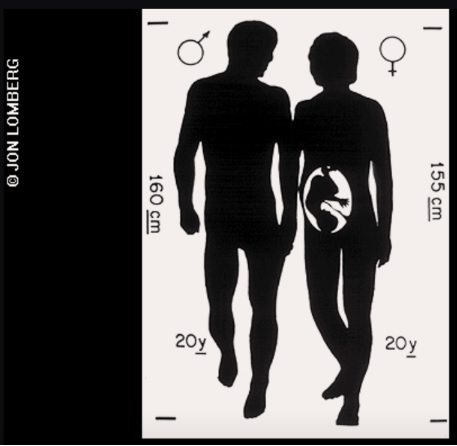
\includegraphics[width=1\columnwidth]{parents_voyager.jpg}
\caption{Two visually distinct life forms, each apparently required for reproduction. Image decoded from the golden disk.
\label{fig:1}}
\end{figure}

\begin{figure}
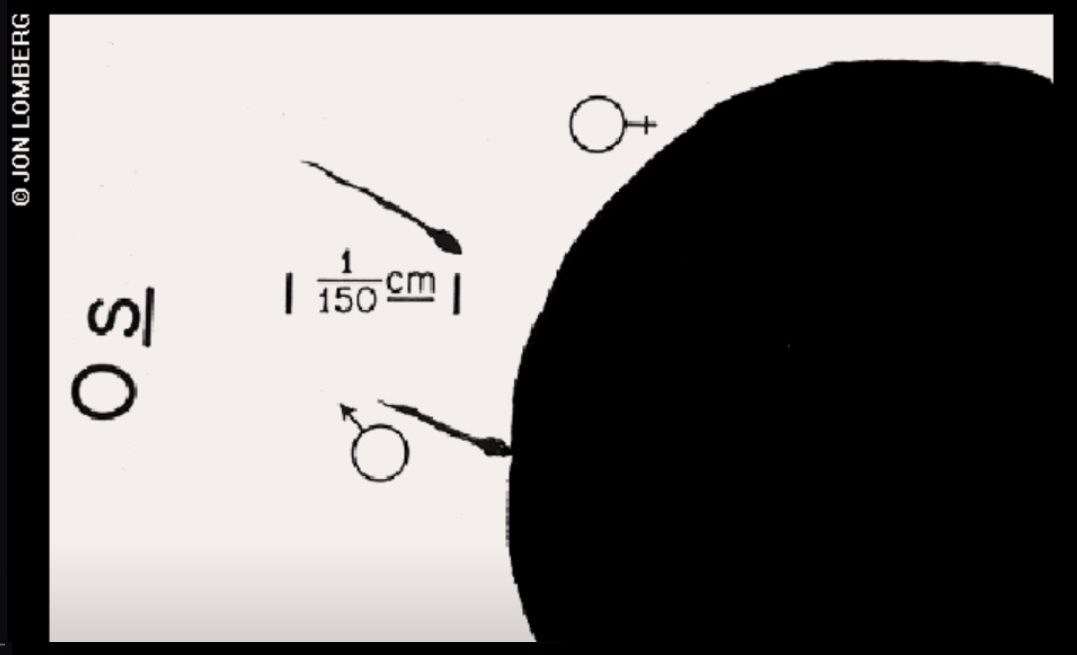
\includegraphics[width=1\columnwidth]{spermandegg_voyager.jpg}
\caption{Entities that are subsets of the life forms depicted in Figure~\ref{fig:1}. These apparently function as the direct mechanisms leading to reproduction and exhibit extremely large size differences. Image decoded from the golden disk.
\label{fig:2}}
\end{figure}

\begin{figure}

\includegraphics[width=1\columnwidth]{rassMandal.jpg}
\caption{Optimal electromagnetic signal receiving structure in Santa Fe, NM.
\label{fig:3}}
\end{figure}


%Again, while we think there are many different points of conversation among our species, the fact that our worlds evolved fundamental differences in reproduction, which then have down-the-line effects for biological family formation, for inequality, species health, and even overarching societal effects (like immigration), we decided to modify our course slightly towards your planet to to understand why you have a two-parent system. Once close enough, we were able to tap into your communication networks and download more information from your planet. We learned many of your languages, watched and read more recordings, and discovered how you humans analyze your own world and its laws, or what you call ``science''. 

%We have 72 hours in your planet's vicinity, and have decided to use this time to send you this report about other planets' reproduction system. In this report, we explored how these systems emerged, how they work biologically, and their societal consequences. We use your scientific writing style and incorporate your own scientific models to make our points more understandable to you.

Several questions still remain regarding your reproductive system. Is this reproductive system limited to ''humans'' or do other organisms also subscribe to two-parent systems? Upon examination of your literature we have determined that most organisms on Earth subscribe to a biparental system, though humans take it to the highest extreme, imbuing societal importance in biparenting. While we have determined that other parental systems among humans exist (for example, what you call polygyny), norms of dominant cultures seem to imbue a superiority to biparenting, even suggesting that single or multi-parenting is deviant and morally inferior. We hope to use the information we send here to suggest that other systems can in fact exist and may in fact imbue certain advantages over biparenting strategies.

In the remainder of this message, we present a series of wide-ranging consequences of the choice of reproductive system, from molecules to societies:

%the following paper we present these ideas scientifically. Below we describe how our system evolved and the implications this has for ecology and society.

\begin{enumerate}
    \item \textbf{The evolution of $n$-parental systems}: In our home star system, which is composed of $N$ planets, all life forms have evolved reproductive systems that require at least three parents. The modal value of parents is 3, though it is possible (and probable) to have more than three parents in our system. Our system is composed of planets that have very limited atmosphere, while your planet has a radiation-protecting ozone. Due to the fact that life on our planets is exposed to, on average, ionizing radiation from 500 to 2,000 Milli-Sievert (mSv), we have higher rates of mutation than life on earth. Due to this, the recombination of genes from multiple parents allows for more viable, and less mutated, life. Recombining genetic material from multiple individuals is highly beneficial in our environment; we are relieved that your planet at least recombines genetic material. Asexual reproduction, we have found, is the worst for offspring and leads to some deleterious mutations out in space!

    \item \textbf{The implications of n parents on ecosystems}: By moving from a 2:1 to a 3:1 parent system, does this reduction in birth rate allow for a slower growth to carrying capacity? What is our population growth in this system?

Having just a replacement rate, you can keep your load on the planetary ecosystem fairly low. So if at a 30 percent marriage rate, and having 3 children, that's replacement rate. This is far below human reproduction rate, which is good.

\item \textbf{The implications of n parents on health}: Three parent systems where parents equally invest in offspring generally lead to greater well-being of children as well as those who gestate the child (what you call the "mother"). In our survey of life on earth we notice that in systems where there are multi-parent systems alongside two-parent system, that multi-parent groups exhibit greater wealth, as well as higher health security for children and mothers.

Despite this, it seems that two-parent systems are the norm. Some seem to suggest it's so that the genetic-material donor (what you call the "father") knows that the offspring is his, while others suggest that the mother drives these two-parent systems, to ensure investment from the father. 

Because of the long-term co-evolution between our high-radiation planet and life, we do not have these same kinds of issues. Equal investment among three parents ensures offspring have low mutation rates, and so each of the N parents are equally invested in their lovely, mutation free, children. 

\item \textbf{Mating selection and Marriage rates}: BLah here.


\item \textbf{How do n-parent systems impact cultural homo/heterogeniety?}: Our interplanetary society evolved to high homogeneity, with mostly one dominant language and culture. However, from the Voyager data as well as other uploaded data from Earth, we notice that your planet has high cultural heterogeneity. A full understanding of this difference between our two civilizations would require more knowledge than is currently possessed about both humanity's deep past are our deep past. However, it this document we present a how-possibly model that points to our system of $n$-partner reproduction, where $n>2$, as a possible explanation for our comparatively high level of cultural homogeneity.

%\textbf{How do n-parent systems impact Health?}: What is the link between std's and mutations? Are mutations lower while STDs higher?

\end{enumerate}

We hope this message will interest you and further your understanding of other possible worlds. 

Peace to all and health forever, 

\chapter*{The Evolution and Consequences of Tri-parental Systems}


\textit{This is a work of speculative science, any resemblance to any civilization is coincidental.}
\vspace{12pt}


Upon examination of your literature we have determined that most organisms on Earth subscribe to a bi-parental system. In this paper, we would like to explain the emergence of tri-parentalism and its consequences. First, we explain in what conditions a tri-parental world might emerge, and when would it include three different mating types (subgroups of individuals in a species, where individuals in one subgroup preferentially mate with those in other subgroups). Second, we describe the genetics of our species which enable tri-parentalism. Third, we give examples of species with a tri-parental system. Fourth, we discuss some implications of this tri-parental system on disease dynamics and family health. Fifth, we investigate how our monoculture might have been a consequence from our tri-parental system. Finally, we investigate the implication for costly signaling, the origin of the biochemistry of our life form, the emergence of monogamous tri-parental marriages, and the meaning of life. 
%The "finally" will be cut off due to transmission ending! 

\section*{The origin of tri-parentalism and three mating types} 

\begin{figure}
\centering
%\begin{wrapfigure}{l}{4cm}
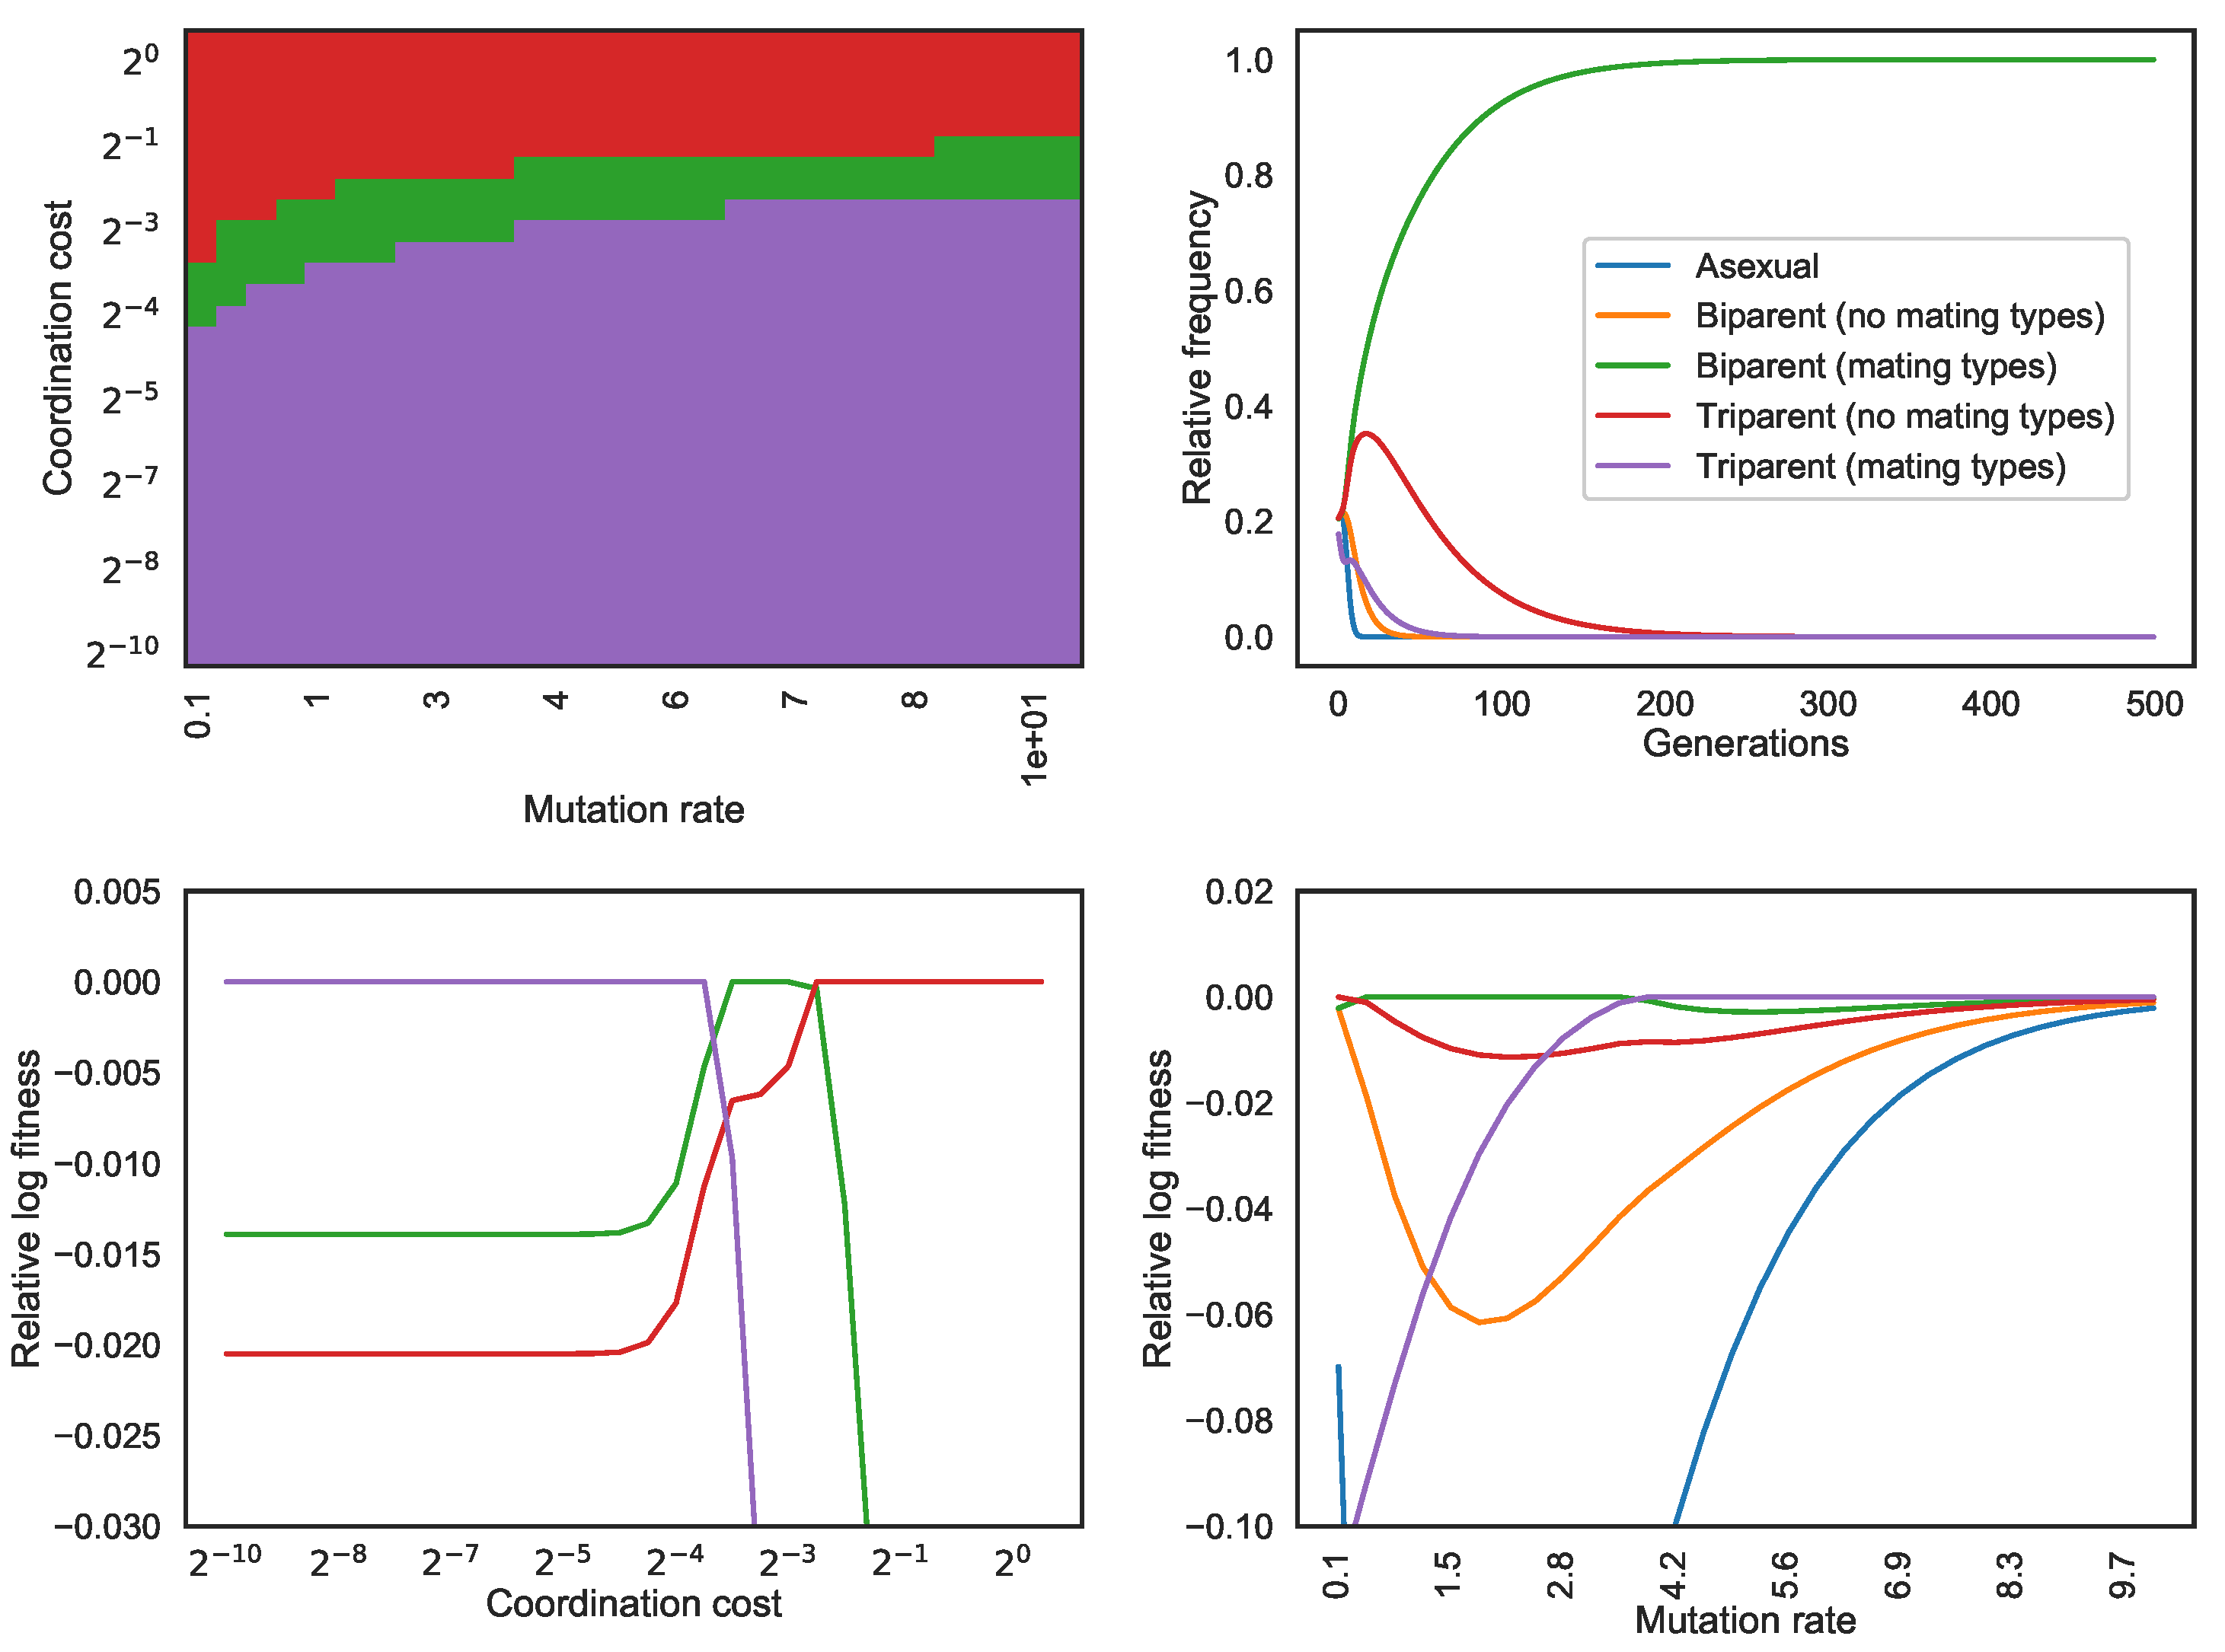
\includegraphics[width=0.9\textwidth]{Artemy/heatmap.pdf}
\caption{Optimality of biparentalism/triparentalism self-avoiding mating types under different conditions. Five mating strategies are considered: asexuality, biparentalism (with and without self-avoiding mating types), and triparentalism (with and without self-avoiding mating types). \textbf{Top left}: Optimal mating mating strategy as a function of mutation rate (average number of mutations in an offspring) and coordination cost (see legend in top right for colors). \textbf{Top right}: Relative frequency of different mating types over the course of evolutionary dynamics. All mating types start with the same frequency, and all individuals start with 0 deleterious mutations.  \textbf{Bottom left}: relative log fitness for different mating types as coordination cost changes (mutation rate is fixed to $\approx 1$). \textbf{Bottom right}: relative log fitness for different mating types as mutation rate changes (coordination cost is fixed to $\approx 2^{-3}$).}
\label{fig:heatmapartemy}
%\end{wrapfigure}
\end{figure}



Both our home planet and Earth have evolved sexual reproduction, such that the production of offspring requires more than one parent. Although there are potential costs of sex (\emph{e.g.}, a ``two-fold cost of males'' for many Earth species \cite{smith2017origin,smith1978evolution}, increase in disease spread, increased coordination and search costs, see later sections), the ubiquity of sex also implies strong benefits. One theoretical model \cite{kondrashov_selection_1982} demonstrated that sex can dilute the number of deleterious mutations in a genome, while asexual organisms monotonically increase their mutational load. This can favor the evolution of sex. 

But how many individuals should combine their genetic material to produce an offspring? On Earth, the overwhelmingly dominant mode is two parents (although there are a very small number of exceptions; \cite{cohen2013biological,bloomfield2019triparental}). On our home star system, three parents is the mode. We discuss in the next section how three parents could combine genetic material to produce an offspring. 

In addition to the number of parents, species may differ in the number of mating types. Mating types are subdivisions of a population where individuals of one mating type preferentially mate with individuals of one or more different mating types. For humans, there exist two mating types (\emph{i.e.}, males and females) but for other organisms on Earth, such as fungi and slime molds, there can be many more mating types \cite{collins1977new}. Our own species happens to have three mating types. The existence of mating types implies the ability to avoid mating with one's own type (self-avoidance). This may be beneficial because it can increase the genetic diversity of offspring, but may also entail search costs and prevent an individual from mating with otherwise suitable mates \cite{bull_combinatorics_1989,iwasa_evolution_1987}. 

We asked what ecological differences between our home star system and the planet Earth could have driven the evolution of different numbers of parents, self-avoidance, and different numbers of mating types. We used the model developed by Kondrashov \cite{kondrashov_selection_1982} and extended by Perry \cite{perry2017sex} to examine the role of mutation rate, encounter rate, and the coordination cost of $n$-parental systems on the emergence of stable bi- and tri-parental systems.


\subsection*{Model of emergence of tri-parental systems} 
For you to understand the origin of our triparental system, it is first helpful to consider the benefit of sexual reproduction in general. It has been observed that a major problem is that with asexual reproduction, deleterious mutations can continuously accumulate. This occurs because it is more likely that an asexual offspring acquires an additional mutation, instead of removing a previously acquired one [Cite Muller]. Among other other advantages~cite{kondrashov1993classification}, sexual reproduction can dramatically increase the variability found among offspring, including variability in the number of deleterious mutations: some offspring will have many more mutations than their parents, and some will have many fewer. Natural selection can then use this variability to favor offspring with few mutations, maintaining in check the overall level of mutations in the population.

Based on these observations, Earth-based scientists created a simple model that explains the benefit of biparental sex in terms of removing deleterious mutations~\cite{kondrashov_selection_1982,kondrashov_deleterious_1988}. Recently, however, researchers realized that triparental reproduction can be even more effective at removing deleterious mutations, and (absent other assumptions) in fact has advantages over biparental reproduction~\cite{perry_why_2017}. As we will see, this ability to very effectively remove deleterious mutations is why triparentalism became dominant in our world.

Importantly, these models~\cite{perry_why_2017,kondrashov_selection_1982} explained the benefit of sexual reproduction without considering what role, if any, may be played by the presence of different mating types (whether symmetric or asymmetric). At the same time, the benefit of sex obviously occurs only when the parents are not genetic clones (otherwise sexual reproduction becomes equivalent to asexual reproduction). In the models of~\cite{perry_why_2017,kondrashov_selection_1982}, however, it is always assumed that parents are not clones of each other. 

This is not adequate for explaining our world. When sexual reproduction originated on our planet, it required only the presence of any three parents, which were not differentiated into mating types (i.e., any organism could in principle mate with any two other ones). The three parents would deposit a large number of gametes into the same pool. In this pool, triplets of gametes would then come together and sexually fuse, thereby forming new organisms. In many cases, however, this scheme did not lead to the full benefits of sex, because the three gametes that would fuse would not always originate from three different parent organisms. In fact, when three organisms contribute gametes to a common pool, there is only a 2/9 probability that a randomly chosen triple of gametes will represent all three parents. Thus, in our original system, sexual reproduction would often invovle the mixing together of clones, in this way loosing some of the advantages of sex (and also violating the assumptions of the aforementioned models~\cite{perry_why_2017,kondrashov_selection_1982}).

To develop self-avoidance —- that is, to not allow sexual reproduction between clones — our life-forms developed a system in which organisms are differentiated into 3 different mating types (which, at this point, were still phenotypically symmetric). A mating event between three parents could only happen if the three parents belonged to three different mating types. Moreover, gamete triplets that came together would only initiate sexual fusion when three different mating types were represented in a triplet. This guaranteed that gametes from the same parent (which would be clones) could never join together. This is the origin of triparental reproduction on our planet, as well as the origin of our three self-avoiding mating types. The asymmetry in the gametes of these three mating types followed later, and is described in more detail below.

The mating scheme described above guarantees self-avoidance, but it is not without some possible disadvantages. In particular, under this system, not all possible parent triplets can mate, but only those triplets that contain all three different mating types. There is only a 2/9ths probability that three parents chosen from a population will contain all three mating types. If a self-avoiding parent only has a single chance to find a set of mating partners, this cost is enormous. However, if such a parent has many possibilities to find a set of compatible mating partners in a given mating period, then this cost decreases (in particular, the probability that an acceptable triplet is found after $n$ attempts is $(1-(2/9))^n$). This can be represented in terms of a \emph{coordination cost}, which is equal to $1/n$.  Coordination cost is the portion of an organism’s mating period that is required to find one possible set of mating partners. It approaches 0 when an infinite number of possible triplets can be attempted in a given mating period (in which case, an acceptable set of mating partners will always be found), and 1 when only a single possible mating triplet can be attempted.

There are many different mating systems possible. The number of parents can be 1 (asexuality), 2 (biparentalism), 3 (triparentalism), or even larger ($n$-parentalism). There can also be different systems of mating types. Furthermore, different mating systems can carry different kinds of costs, such as the coordination cost that define our self-avoidance scheme. Using a simple extension of the models mentioned above~\cite{perry_why_2017,kondrashov_selection_1982}, we show that different kinds of mating systems are favored under different conditions (these results are summarized in \cref{fig:heatmapartemy}). In particular, across the parameters considered by our analysis, there is a sequence of optimal schemes going from (1) a triparental system with no mating types to (2) a biparental system with self-avoiding mating types to (3) a triparental system with self-avoiding mating types (our system). Generally, system (1) is favored when coordination costs are high and/or when mutations rates are low, and system (3) is favored when coordination costs are low and mutations rates are higher. In transitions from (1) to (3) there is always a region in which a self-avoiding biparental system becomes optimal. Note that $n$-parentalism for $n>3$, either with or without self-avoiding mating types, can also be favored, though for simplicity we do not analyze its dynamics here. 

\subsection*{Mutation and coordination in finite populations}
The above model assumes an infinite population and is limited to species with asexual, bi-, or tri-parental reproduction. This leaves a number of question unanswered. For one, does tri-parental reproduction dominate all $n$-parental reproductive strategies, or is it dominated under some circumstances by reproductive strategies with more parents? Moreover, the above model assumes infinite populations. Is this assumption critical to its results?

To address these questions, we implemented Kondrashov's model of deleterious mutations as an agent-based model. Each population consisted of a finite number of organisms who reproduced either bi-, tri-, or quadri-parentally, defined as the number of gametes that are required to produce an offspring. 

Species could also engage in self-avoidance, such that any individual could only contribute one gamete to an $n$-parental offspring. Said otherwise, in a self-avoiding $n$-parental species, all $n$ gametes must come from $n$ unique individuals. In the absence of self-avoidance, for example, offspring in a $3$-parental species could be produced from the gametes of only two individuals, with one parent supplying two gametes (i.e., a kind of hybrid sexual-asexual reproduction). In concrete terms, one might imagine a well-mixed urn into which $n$ parents had contributed an arbitrarily large but equal number of gametes. In the absence of self-avoidance, any $n$ gametes could be drawn at random from the urn to create an offspring. With self-avoidance, gametes from $n$ unique individuals would need to be drawn from the urn to create a viable offspring. If repeatedly drawing gametes from the urn is costly, then self-avoidance would incur a `coordination' cost, which would increase monotonically with the number of self-avoidant parents involved in reproduction.

In this model, a 3-parental mating strategy once again dominated the 2-parental strategy. But the 4-parental strategy dominated the 3-dominated strategy, the 5-parental strategy dominated the 4-parental strategy, and so on. This monotonic dominance hierarchy, however, was disrupted by the cost associated with finding gametes from $n$ unique individuals. Indeed, under reasonable assumptions about the cost of coordinating the gametes of $n$ unique parents, tri-parentalism actually dominated both bi-parentalism and quadri-parentalism (and thus all forms of $n$-parentalism with $n>3$). 

\begin{figure}
    \centering
    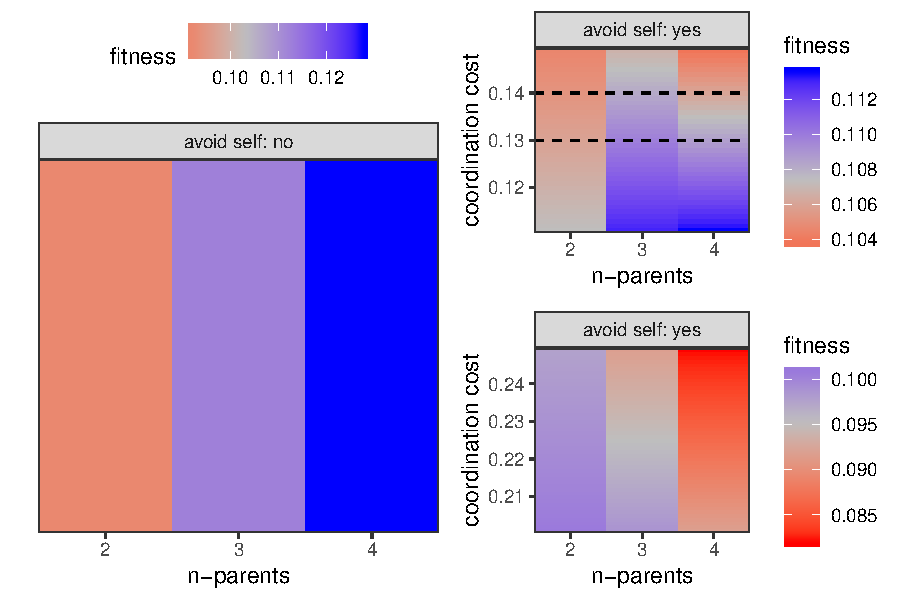
\includegraphics[width=0.9\textwidth]{TylerFigures/tyler72plot.pdf}
    \caption{Relative success of $n$-parental reproductive strategies, with and without coordination costs. Dashed horizontal lines demarcate the coordination costs in which 3-parentalism dominates other $n$-parental reproductive strategies.}
    \label{fig:tylerModel}
\end{figure}

Thus, in finite populations of self-avoiding organisms in which there are costs associated with coordinating the reproduction of $n$ unique organisms, there is a sweet spot where the benefits of combining the genetic material of $n$ unique parents outweighs the cost of coordinating the combination of those parents. Under reasonable assumptions, the optimal value of $n$ is 3. It is possible that the Earth's unusual combination of low mutation rates and high coordination costs could have created an environment for bi-parentalism to thrive, despite its obvious shortcomings.

\subsection*{The evolution of self-avoiding mating types in sexually reproducing species}


While we can establish that there are cases where self-avoiding mating types outperform a system where any three (or two) individuals can reproduce, it is less clear how self-avoiding mating types might initially emerge in a sexually reproducing population. Although this remains an open question, a negative result in our own scientific literature provides an intriguing lead in this direction. This study used an agent based model to simulate a spatially structured population of individuals depositing gametes into a local pool. Similarly to the mathematical model above, each gamete contains a single chromosome, represented by a string specifying whether each site contains a wild type allele or a deleterious mutation. When three gametes combine to form a new individual, each site has a small probability of a new mutation. All mutations are assumed to be double-recessive i.e. only expressed if zero wild type alleles are present. As above, an individual’s probability of survival decreases with number of expressed mutations. 

At each time step, each individual deposits gametes locally, moves with fixed probability, and dies with fixed probability. Gametes, which are assumed to mix on a smaller spatial scale than individuals, also have a fixed probability to be removed from the pool at each time step. New births occur up to local carrying capacity, using sets of gametes selected uniformly at random from the pool.

Each individual’s gametes are tagged by a type, chosen uniformly from the types of the parental gametes with a small chance of mutation to a novel type. The probability of a gamete rejecting a proposed match in favor of remaining in the pool is a heritable quantity between zero (not self-avoiding) and one (completely self-avoiding), copied from the same parent as the gamete type, and also subject to small mutations. In the initial population, all individuals have no deleterious mutations, are of identical type, and are non-self-avoiding.

Within what the authors acknowledged was a relatively narrow range of parameters, the mutational costs of self-fertilization did not appear to be a strong enough pressure to drive the evolution of self-avoiding mating types. However the authors did mention in passing that, in the course of debugging their model, it seemed like multiple mating types were established and maintained with increasing self-avoidance over time in a (at the time considered to be unrealistic) two-parent, diploid system. Due to our current distance from our home planet, communications will not reach the corresponding author until after our window of communication with earth has closed, but further explorations on this topic would be a rich avenue for future study.


\section*{The genetics of a tri-parental species} 

In this section, we will focus on explaining our genetics and how it compares to the genetics of your species. The details of the origin of the biochemistry of our life form, as well as the precise chemistry that forms it, will be discussed in a later section. For this reason we will refer to our genetic material as sets of double stranded chromosomes when necessary so that you are able to understand the analogy. The main distinction however, is that unlike your diploid genomes, where you inherit one copy of each chromosome from one of your two parents, our genome is triploid, where we inherit one copy of each chromosome from one of our three parents. In both our systems we have gametes: cells used during sexual reproduction to produce a new organism (\emph{e.g.}, sperm or egg in Figure \ref{fig:2}). The details of the recombination events occurring pre-gamete formation are discussed in the `genetics' section of the Supplementary Materials and an overview is shown in Figure \ref{fig:cross3}.

The dynamics of our genetics and how it affects assignment of mating types is surprisingly analogous to yours but with some key differences which will be expanded upon in the SI. As discussed previously, our species is composed of three mating types. These mating types are distinguished by three sex-determining genotypes: `XXY', `XYY' and `XYZ'.
% the quote marks look weird when compiled and i don't know how to do that
Each of these mating types produce haploid gametes, and all three gametes need to come together in order to produce a triploid off-spring. Each parent thus contributes a third of its genetic material to the offspring and conversely the offpring's genome is composed of a third of each of its parents genome.

The XYZ mating type produces the largest gamete, that is then fertilized by the other two smaller ones. In your species, you would thus define XYZ as female and the other two as different types of males, although it is important to note that this analogy does not quite match with our genders. The main difference to note is that the two `male' mating-types each produce only one type of gamete. The XXY genotype only produces X gametes while the XYY genotype only produces Y gametes. It follows that the female, producing all three X, Y and Z gametes, is the one that biologically determines the mating type of the offspring. We have included an example of the "Punnet square" that describes sex determination in the case of two types (Table \ref{tab:punnet_human}) and its extension to illustrate this concept in our species with (Table \ref{tab:punnet_us}). In the next section, we discuss models for the emergence of these asymmetrical gametes (when gametes evolve different size characteristics). 

\begin{figure}
\centering
%\begin{wrapfigure}{l}{4cm}
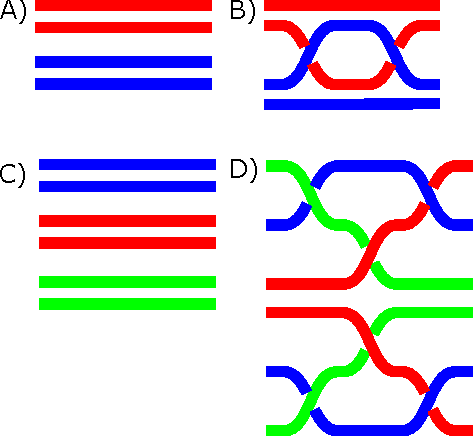
\includegraphics[width=0.4\columnwidth]{AshleyFig/cross_3.pdf}
\caption{A) Illustration of Earth based diploid genome. B) Chromosomal crossover during meiosis in diploid system. C) Result of crossover in diploid system. D) Illustration of our triploid genome. E) Chromosomal crossover during meiosis in triploid system. F) Result of crossover in triploid system.}
\label{fig:cross3}
%\end{wrapfigure}
\end{figure}

%\begin{table}
%\centering
%\includegraphics[width=0.3\columnwidth]{AshleyFig/punnet.pdf}
%\caption{A) Punnet square of mating type assignment in humans. B) Partial Punnet cube of mating type %assignment in our species. Letters a, b and c are used to help follow the three-mating types.
%\label{tab:punnet}}
%\end{table}

\begin{table}
\centering
\begin{tabular}{ |c| c c| } 
\hline
& $X$ & $Y$ \\
\hline
$X$ & $XX$ & $XY$ \\ 
$X$ & $XX$ & $XY$ \\ 
 \hline
 \end{tabular}
\caption{Punnet square of mating type assignment in humans.} 
\label{tab:punnet_human}
\end{table}

\begin{table}
\centering
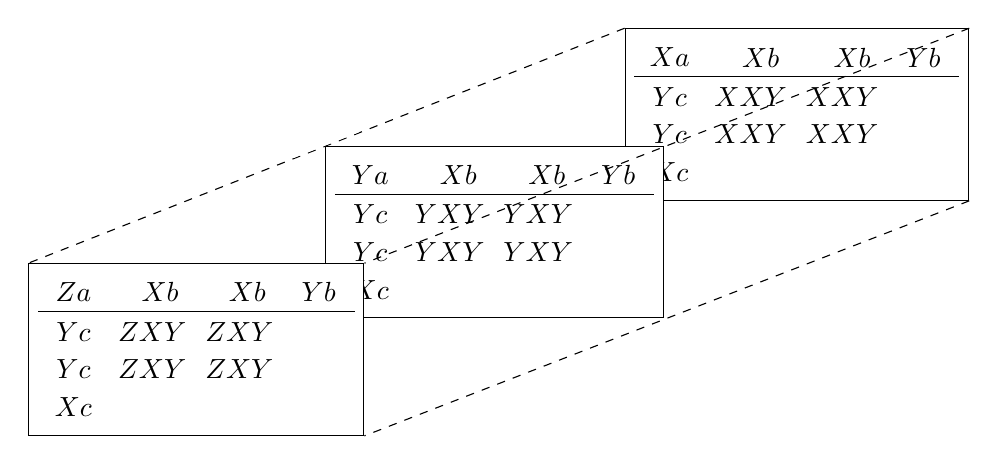
\begin{tikzpicture}[every node/.style={anchor=north east,fill=white,minimum width=.9cm,minimum height=.9mm}]
\matrix (mA) [draw,matrix of math nodes]
{
Xa & Xb & Xb & Yb \\
\hline
Yc & XXY & XXY &  \\
Yc & XXY & XXY &  \\
Xc &  &  &  \\
};

\matrix (mB) [draw,matrix of math nodes] at ($(mA.south west)+(.5,0.7)$)
{
Ya & Xb & Xb & Yb \\
\hline
Yc & YXY & YXY &  \\
Yc & YXY & YXY &  \\
Xc &  &  &  \\
};
x
\matrix (mC) [draw,matrix of math nodes] at ($(mB.south west)+(.5,0.7)$)
{
Za & Xb & Xb & Yb\\
\hline
Yc & ZXY & ZXY &  \\
Yc & ZXY & ZXY &  \\
Xc &  &  &  \\
};
\draw[dashed](mA.north east)--(mC.north east);
\draw[dashed](mA.north west)-- node[sloped,above] {} (mC.north west);
\draw[dashed](mA.south east)--(mC.south east);
\end{tikzpicture}
\caption{Partial Punnet cube of mating type assignment in our species. Letters a, b and c are used to help follow the three mating types.} 
\label{tab:punnet_us}
\end{table}



\section*{The emergence of gamete asymmetry in tri-parental systems}
\begin{figure}[htb!]
    \centering
    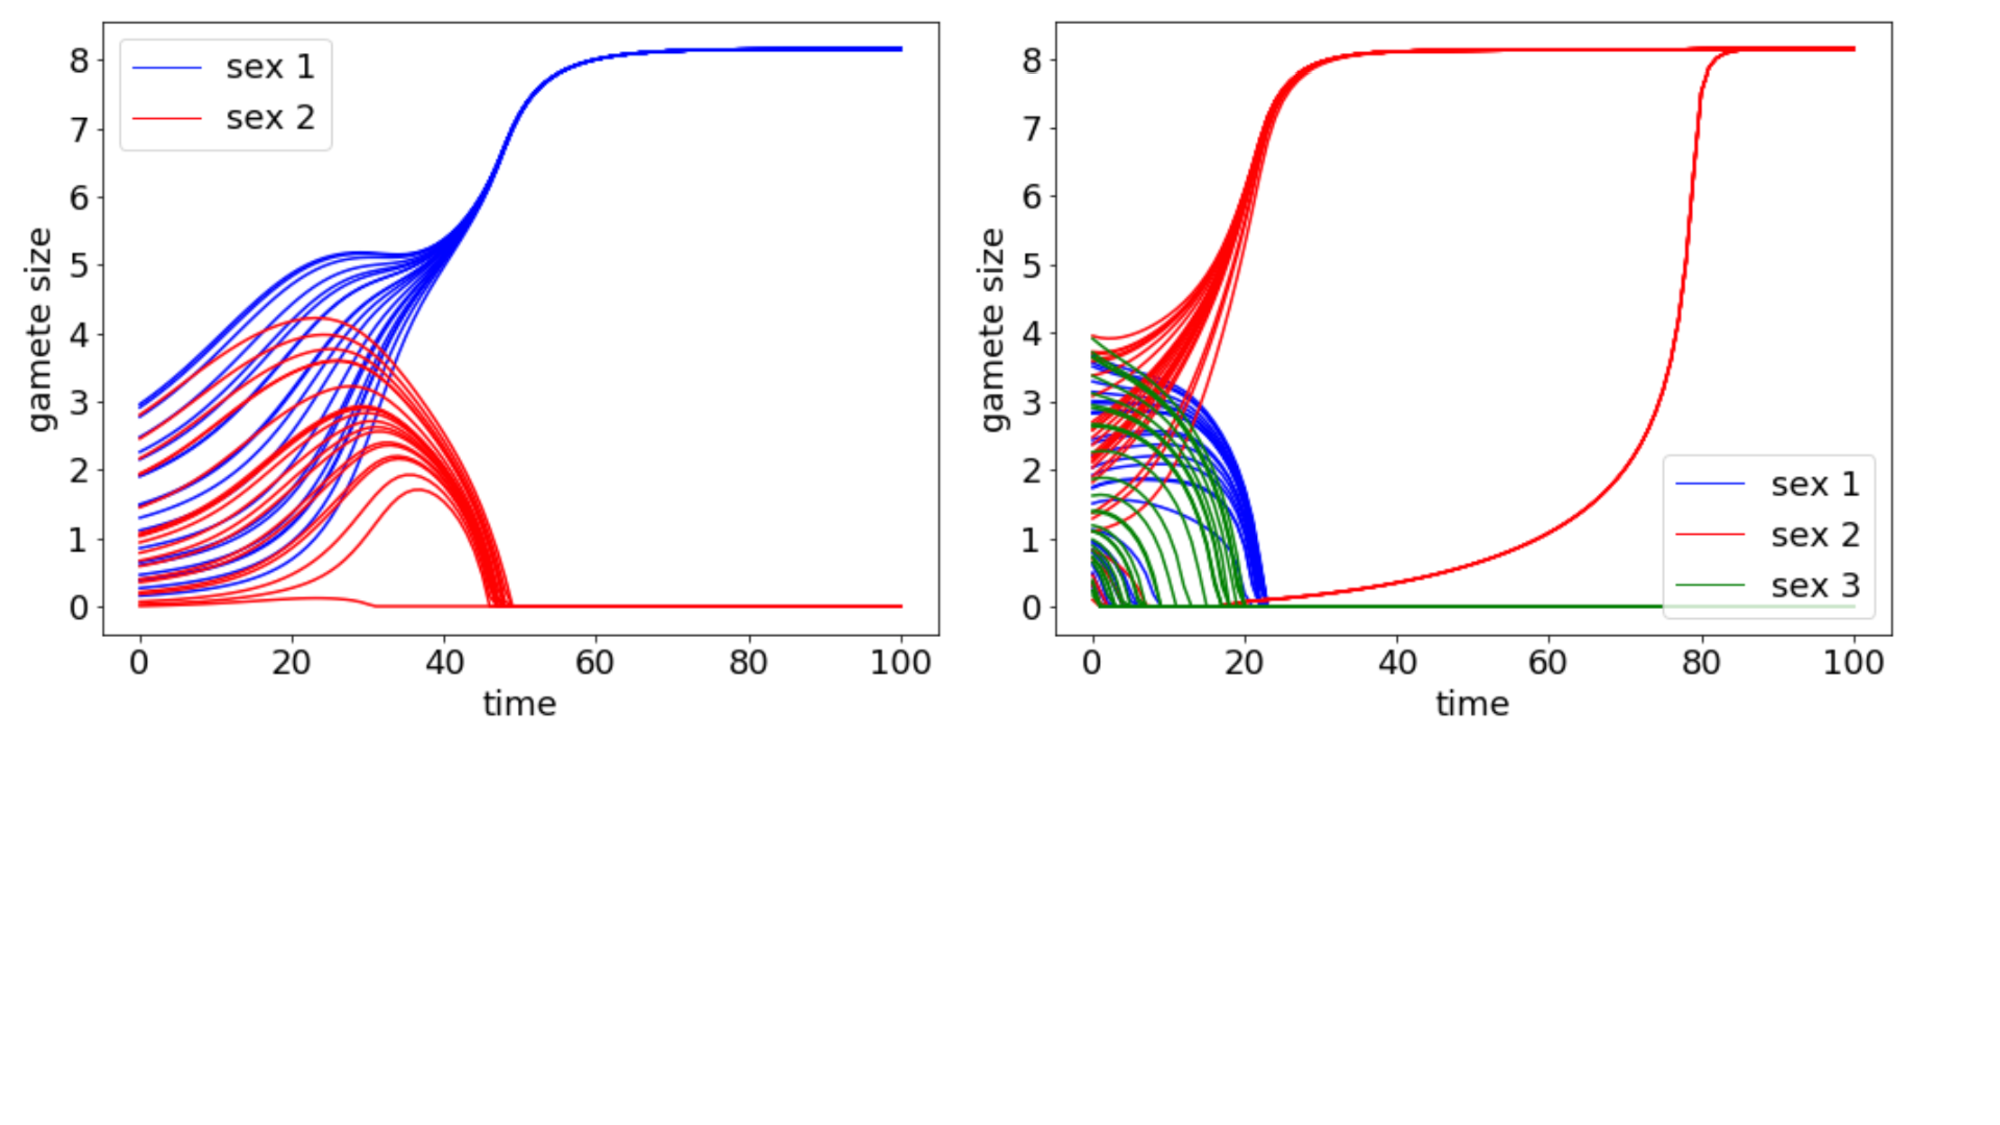
\includegraphics[width = 0.9\textwidth]{vickysFigs/2panels}
    \caption{Simulation for the gamete size evolution. The colors distinguish gametes of different sexes. Each curve indicates the evolution trajectory of one initial condition in gamete size. Left: in the case of two sexes, one sex evolves to have the minimal gamete size ($0$), and the other sex evolves to have a large gamete size. This recovers what happens on Earth. Right: in the case of three sexes, one sex evolves to have a large gamete size, and two evolves to have the minimal gamete size.}
    \label{fig:gameteSize2Panel}
\end{figure}
The natural history of Earth and our planet differ in many, but not all, respects. Notably, on both Earth and our planet mating types preceded gamete asymmetry. The preceding sections describe the evolution of tri-parental inheritance, mating types, self-avoidance, and genetics in the high radiation environment of our planet. In this section we discuss the evolution of gamete asymmetry, then in the next section link these ideas to the natural history and evolutionary ecology of the species on our planet. These ideas will continue to be pertinent in the sections on society.

As on Earth, there is great diversity in mating systems corresponding with great diversity in fertilization strategies. Nevertheless, the modal mating system has three self-avoiding sexes. Furthermore, the most common pattern for gamete sizes on our planet, as described above, is for two sexes to produce gametes near the minimum viable size, while one sex produces much larger gametes. However, an important minority of species have one sex that produces gametes near the minimum viable size, and two sexes that produce larger gametes. Since on Earth sexes with small gametes are usually called male and those with large gametes female, it is perhaps tempting to associate all small gamete sexes with male and large with female. This is probably useful, but certainly masks a great deal of nuance, especially since our social scientists also make a similar distinction as yours between sex and gender.

To make these ideas concrete, we present both a dynamic and static model of the evolution of gamete asymmetry, both of which take three self-avoiding mating types with distinct gametes as given. These are both described in full detail in the SI. The dynamical model assumes a coupled system of multiple sexes evolving together. The model assumes that the gamete sizes of all sexes evolve via natural selection to increase the number of off-spring that individuals have. The number of off-spring depends on two components. The first is competition with members of own-sex, where the chance of one's own gamete successfully merging with that of one's mate(s) increases with the number of gametes produced; however, there is a trade-off in the total energy used for gamete production, so that producing more gametes comes at the cost of lower gamete size. The second component is cooperation with other sexes, where the chance of the off-springs being born successfully increases with the size of the two merged gametes. We perform an agent-based simulation for this model, and the results are shown in Figure~\ref{fig:gameteSize2Panel}. To convince you of the model's validity, we show that the two-sex case of the model recovers what we observe is typical for Earth --- one sex evolves to have a large gamete size, and the other evolves to have the minimal gamete size. In the three-sex version of the model, we show that one sex evolves to have a large gamete size, and the other two evolve to have the minimal viable gamete size. 

The second model reaches an almost identical conclusion, albeit with different theoretical machinery. In particular, we assess the evolutionary stability of tri-parental inheritance with three mating types for which each mating type has exactly one distinct gamete. For the Flying-Flower species discussed in more detail below, we provide conditions so that it is an evolutionarily stable strategy (ESS) for two species to adopt a minimum viable gamete size, and one to adopt a large gamete size. That is, the minimal gamete size of two sexes are found to be a corner solution of the optimality condition and mutating them to a larger size would not improve their fitness. When the two sexes exhibit minimal gamete sizes, the large gamete size of the other sex is also evolutionarily stable. These conditions have to do with the probability of double matings. So long as these probabilities are even slightly above zero, the ESS exists. With slight modifications, this model works for most species on our planet (including us), though as we point out above there are species with sufficiently unique mating systems such that other ESSs exist.

% Mike: One attempt at Victorian language:
\section*{Some illustrating examples from the natural history of our planet}
%\section*{The evolutionary ecology and sociobiology of tri-parentalism}
As on your world, gamete asymmetry has had far-reaching consequences on the subsequent development of species that evolved it. This is easiest understood by loosely associating sexes having small gametes with Earth males and sexes having big gametes with Earth females, though, as pointed out above, much nuance is lost by making analogies with Earth sexes. To summarize core, relevant points made above: (1) the most common gamete pattern on our planet is small/small/large and (2) amongst sexually reproducing species the ancestral (and most common) mating mechanism involves three sexes coming together at one place to fertilize an egg with three gametes. Our species follows both of these dominant patterns: small/small/large gametes and three-sex mating events. We do discuss, below, an interesting case of a species that does not follow the three-sex mating event pattern.

It is common on our planet for ``males'' of a species to evolve flashy displays as the result of sexual selection. Similarly, males of some species maintain harems and thus have evolved substantial physical dimorphism. One phenomenon that some species on our planet exhibit, that could not emerge on your planet, is frequent cooperation in seeking mates between individuals of the ``male 1'' sex and ``male 2'' sex. This is possible because these males are not competing directly with each other for genetic heritage, but do share a common interest in reproducing with ``females.'' It is common in such species that males of one sex are relatively small but specialize in costly display (see the section below on costly signaling) whereas males of the other sex are drab (both physically and behaviorally) but grow large or otherwise evolve exceptional physical characteristics, such as great agility or stamina. Clearly, the consequences of tri-parental inheritance and gamete asymmetry are sufficiently far-reaching that we cannot address all of those consequences here. In lieu of that, we unpack one particular case study in greater detail: the Flying-Flower genus (this our best attempt at a literal translation of our name for this set of species).

In Earth idiom, Flying-Flower species are a textbook example in our world. Indeed, they are taught formally to the juveniles of our species as a touchstone example in biology and ecology. For this reason, it is the mating system analyzed in the SI and discussed in the preceding section. Flying-Flower species follow the more common gamete pattern of our planet (small/small/large), but do not follow the more common pattern of simultaneous three-sex mating events. What is perhaps most notable about Flying-Flower species is that the three sexes have very different physical structures and behaviors. The so-called Flower sex ($F$) is sessile and, like plants on Earth, photosynthesizes. The other two species are the Pollinator ($P$) and Central species ($C)$. The Pollinator transfers genetic material from $F$ to $C$, but unlike with Earth pollinators, who typically receive a food reward such as nectar, its ``reward'' is that it mixes in its genetic material with the genetic material of $F$. For much of our history, our scientists assumed that the three sexes of species in the Flying-Flowers clade were distinct species because of their great physical and behavioral differences. It was a watershed moment when our scientists realized that, in fact, they consist of members of the same species. Indeed, this insight led three of our scientists to independently and near-simultaneously discover the principle of natural selection, much as Charles Darwin and Alfred Wallace co-discovered natural selection at nearly the same time in your world.

Individuals of the sessile $F$ sex compete for the attention of the pollinating $P$ sex by creating flashy, decorative bundles containing their genetic material. The pollinators, $P$, do not need to engage in costly display because the more fit individuals are more adapt at gathering the best bundles. Thus, their ability to gather high quality display bundles is a direct, honest reflection of their quality. The pollinators add their own genetic material to their display bundle, then display it to individuals of the central sex, $C$, who choose which bundle to accept and use for reproduction. It is rare for either $F$ or $P$ individuals to engage in substantial parental investment. As a closing note for this case study, we have observed a similar phenomenon among Flying-Flower species (and other species on our planet) to what you call the Trivers-Willard hypothesis: high quality members of the $C$ sex will invest greater parental effort in the sex or sexes with the higher variance fitness outcomes ($F$ and/or $P$), whereas low quality $C$ individuals will invest greater parental effort in the lower variance sex or sexes.
%but for our most common gamete pattern (two small, one large) one is well-served by associating the small gamete sexes with Earth males and the large gamete species with Earth females. In Earth terminology this would be called a text-book example since 

%(a core topic in your field called evolutionary ecology), and the tri-parental inheritance system clearly  kin-selection in ways that are laid out below

%the evolutionary ecology and sociobiology of species across the planets of our solar system. 

%However, an important minority of species have one male-like sex and two female-like sexes or adopt sex-roles that are difficult to associate with Earth types. 

%Species in the Flying-Flowers clade have three sexes with very different physical structures and behaviors. The so-called Flower sex ($F$) is sessile and, like plants on Earth, photosynthesizes. The other two species are the Pollinator ($P$) and Central species ($C)$. The Pollinator transfers genetic material from $F$ to $C$, but unlike with Earth pollinators, who typically receive a food reward such as nectar, its ``reward'' is that it mixes in its genetic material with the genetic material of $F$. For much of our history, our scientists assumed that the three sexes of the Flying-Flowers clade were distinct sexes because of their great physical and behavioral differences. It was a watershed moment when our scientists realized that they were

%Like the Flying-Flowers, our species has two sexes with small gametes and one with large. However, unlike with the Flying-Flowers, mating occurs as one event among three individuals of each sex, not via two distinct mating events that occur between two sexes ($F$-$P$ and $P$-$C$).

\section*{Disease transmission dynamics in a tri-parental reproduction process}



\section*{The implications of tri-parentalism for society}

We review a few implications that a tri-parent system would have on greater social structures. We believe there are many consequences beyond this paper, but concentrated on two different, interrelated outcomes:\ marriage rates, and the presence/absence of cultural diversity.

\subsection*{Matching model: marriages and divorce}

Marriages have emerged across cultures as recognized unions between two or more individuals \cite{Fortunato2015}. While marriage does not require or assume reproduction, it does often involve restrictions on sexual relations and investments in children. On earth, there are usually three configurations: 1) monogamous marriages (a person only has one spouse at a given time), 2) polyandry (a female has multiple male spouses at any given time), and 3) polygyny (a male has multiple female spouses). While polygyny (a male with multiple female spouses) is historically the default human marriage system, monogamy has emerged in situations where more control of inheritance is needed \cite{Fortunato2015, Fortunato2009}. 

Our society does share marriage as an institution, and tri-person monogamous marriages have become the norm. However, the difference in the number of sexes to be matched seems to have resulted in salient differences between our institution and yours. From what we observed in your fictional stories, it seems that your marriage is very stable, or at least aims to be so. In your ``movies'' and ``drama series'', we have observed that couples frequently declares ``eternal love'' and they decide to ``live happily ever after''. 

Our system of marriage does not work that way. Marriages among our species are typically much more short-lived than marriages among humans on Earth, and most parties to a marriage do not anticipate that it will last for the remainder of their lifetime. Our people repeat getting married, getting divorced, searching for better mates, getting married, etc. This difference is explained by the difficulty of finding the optimal mates in our tri-parental system. Imagine we have a population consisting of $N$ individuals of each mating type. In a bi-parental system, you only need to find a ``soulmate'' from $N$ members of the opposite sex (or, somewhat less commonly, of the same sex), which is ridiculously easy in our ``eyes.'' For us, the perfect match is a ``soul-triplet'' and we each have to find it out of $N^2$ combinations if we are to marry, to use paraphrase your idiom, ``'til  death do the three of us part''. Sadly, this happens only exceedingly rarely.

Figure~\ref{fig:married_rate} demonstrates this point via a simple model. In this model, people from each mating type randomly meet, and form a marriage so long as the marriage improves the pair's/triple's current situation. If we repeat this process infinitely, it should converge to a stable equilibrium. As you can see, the marriage rate at a given time from the start of the model run decreases with more sex types, and the average utility tends to be lower as a result.
\begin{figure}[htb!]
    \centering
    \includegraphics[width = 0.4\textwidth]{hajimeFigs/married_rat4_n.png}
    \includegraphics[width = 0.4\textwidth]{hajimeFigs/average_uti4ity_n.png}
    \caption{The ratio of married population and the average utility.}
    \label{fig:married_rate}
\end{figure}

Note that this model only illustrates the comparative difficulty of finding a mate in marriage systems with different numbers of partners. In reality, we have excellent meeting technology (i.e., dating platforms) tailored to our three-part institution of marriage to facilitate finding a better partner; this makes meeting easier, but does little to change the high divorce rates that typify our species.

Also, marriage in our system is actually slightly more stable than this simple model, due to the desire to avoid paying the search cost in looking for a new triple, and the due to the demands of parental care. However, the fact that achieving a sustainable marriage has low probability has had crucial consequences in our society, particularly with regard to cultural homo/heterogeneity, which we discuss in the following section.

To note, on Earth, there is little evidence that polygyny is harmful for individuals \cite{Mulder1990, Sear2002, Lawson13827}. In societies where monogamy and polygyny occur, polygynous groups seem to lead to greater child and woman health and security \cite{Mulder1990}. Generally speaking, polygynous households are correlated with greater wealth; whether on earth this is due to the fact that wealthier men can have more wives, or those with more wives can aggrandize, is unclear. However, the ``polygyny-threshold model'' suggests that polygyny will develop when costs associated with sharing a husband can be offset by resource accumulation that would be difficult under monogamy \cite{Lawson13827}. What is clear from these studies is that \textit{there is little evidence} that a three- or more-parent group would lead to a decrease in child, mother, or father health \cite{Lawson13827, Mulder1990}. Rather, it seems that evidence points to higher health indices for each individual in this type of family on your own planet.

\subsection*{Cultural mixing under tri-parental reproduction}
The Voyager data, as well as other data that we have uploaded from Earth during our fly-by, strongly suggests that contemporary Earth society is still highly divided into different cultures. This strikes us as surprising; when our society reached Earth's current level of capability for inter-cultural mixing, a homogeneous quickly emerged. In light of the salience of two-parent reproduction in our study of Earth, we chose to investigate whether our own capacity for $3$-parent reproduction can explain, at least in part, the emergence of cultural homogeneity in our society, as compared to the Earthling's highly diverse and stratified system of cultures.\par 

Our model (provided in the SI) shows that under 3-parent reproduction, the average number of cultural affinities that a person can expect to have over the course of their lifetime increases rapidly throughout the generations. At some point, the cognitive load of maintaining multiple cultural identities becomes overwhelming, even for beings like us. We hypothesize that our current cultural homogeneity emerged as a response to the explosion in cultural identities modelled above. This is due to three factors:\ our aforementioned lower rate of people who are never married, the greater possibility for acquiring additional cultural affinities through marriage, and the fact that under 3-parent reproduction, the average number of cultural affinities that a person is born with increases rapidly through the generations. Indeed, as shown in Figure \ref{fig:cultureplot}, our model is consistent with an outcome in which the average person's expected lifetime cultural affinities increases rapidly with their marriage-independent cultural affinities.\par 

\begin{figure}[htb!]
    \centering
    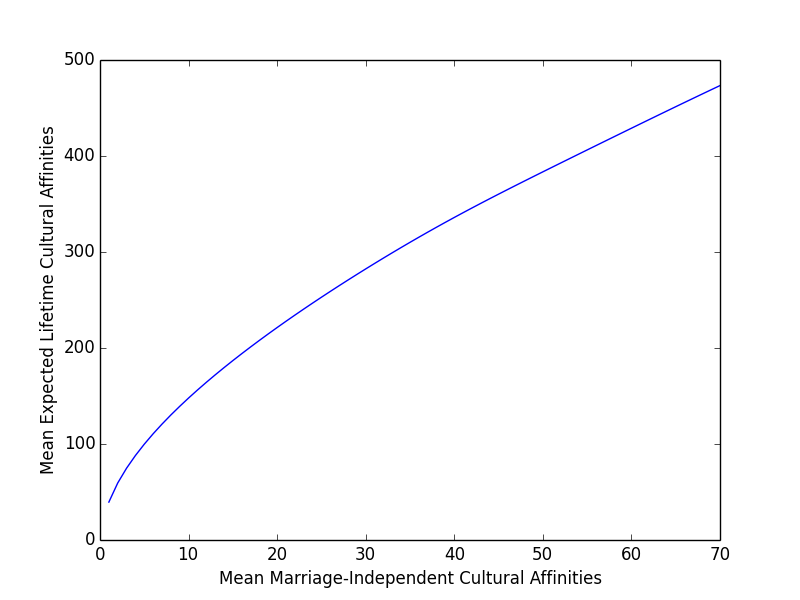
\includegraphics[width = 0.5\textwidth]{culture1.png}
    \caption{As the mean number of cultural affinities that a person acquires outside of marriage increases, the number of cultural affinities that the average person can expect to acquire over their lifetime also increases.}
    \label{fig:cultureplot}
\end{figure}


Certainly, the evidence from Earth suggests that there is a critical level of cultural complexity at which individuals become overburdened and the adoption of a single culture becomes necessary. In an ethnographic study of a highly multilingual after-school program in Los Angeles, \cite{orellana2016cultivating} find that despite speaking a wide array of languages and dialects at home, children in the program converged on a narrower range of English and Spanish dialects when speaking with each other. Data from \cite{rumbaut2013immigration} show that while the United States is historically a country with a high rate of immigration and therefore a rich diversity of language forms, is also a ``language graveyard'', i.e.\ a country where immigrant languages increasingly fall out of use. These findings suggest that there is a level of linguistic diversity at which languages start to fall out of use, due to the need for assimilation. There is some evidence that this is due not just to the desire for assimilation into the dominant community, but also due to the cognitive load of speaking multiple languages. \cite{matras2000fusion}
finds that speakers of multiple languages often develop strategies for ``fusing'' their spoken languages in to one common language, so that the multilingual subject effectively speaks a single, fused language. This fusion develops as a shortcut for avoiding the cognitive load associated with maintaining fluency in two completely different languages.\par 





Language is, of course, only one aspect of culture, and the cultural homogeneity of our current society encompasses more dimensions of culture than language. Indeed, most people in our society speak a common language (aside from our solitary "Turkish" speaker in our voyaging group), but we also share a broader set of common cultural practices. We suspect, however, that the emergence of such cultural homogeneity began with the fusing of language, which led to a broader fusion of cultural elements communicated via a common media. We also have strong evidence that this process of cultural convergence developed at a much faster rate in our society than the rate at which it is currently developing on Earth. In light of the model proposed above, we have reason to suspect that our $3$-participant system of marriage and reproduction, as opposed to a two-participant system, plays a significant explanatory role with respect to the higher rate of cultural convergence that we experienced in our deep past.\par 





Indeed, our antiquarians -- our best translation of a group of social scientists comprising, in your terminology, comparative linguists, archaeologists, historians, and so forth -- have uncovered good, albeit indirect evidence supporting the perspective outlined above. As with your species, the adoption of food production was a seminal moment in our history, leading to the growth of ``urbanism'' and a rapid increase in technological innovation. Prior to this, our ancestors had spread across the continents of our world, developing distinct local cultural traditions, with physical boundaries usually demarcating the cultural boundaries between these groups. Shortly after the adoption of food production, we domesticated a beast of burden (quite unlike your horses, but serving the same functional role) that allowed more rapid movement and vastly expanded trading in material goods as well as the movement of members of our species among previously isolated locations.

This created a set of natural experiments whereby previously non-mixing groups with distinct (and locally unified) cultures came increasingly in contact. Our antiquarians have fused linguistic data with archaeological data -- for the latter, we rely heavily on stylistic differences in vessels created from highly pliable soils fired at high temperatures (similar to your pottery, which we also invented) -- to show that as these natural experiments played out there was a very rapid unification of cultures. This occurred far more rapidly than the most comparable examples from your history, although it was far more difficult for us to piece together the story since differences in atmospheric chemistry between our worlds means we cannot utilize radiocarbon dating, since is not a constant production of carbon-14 from nitrogen-14 in our world. Instead, we utilize less precise and radioisotope dating techniques and largely continue to operate in the regime that some of your archaeologists identify as cultural history. That being said, seriation techniques that form the basis for (relative) dating in cultural history are more reliable in our world since culture change is more rapid.


\section*{Hyperdrive technology, the unified theory of physics, and the meaning of life}

We have, thus far, focused on the implications of a tri-parental system, from the structure of our genetic information, to the evolution of self-avoidance, emergence of gamete asymmetries, spread of sexually transmitted diseases, and social effects from marriage to cultural mixing. 

We now move on to other topics that may be of interest to humans on Earth. We will begin with a detailed description of our hyperdrive technology that allows us to travel at the speed of light, then describe the missing pieces of your understanding of the physical world, and end with the implications of the unified theory of physics on the meaning of life.

Our hyperdrive technology is based on the well-known phenomenon of... 

\section*{Costly signaling}
\begin{figure}[htb!]
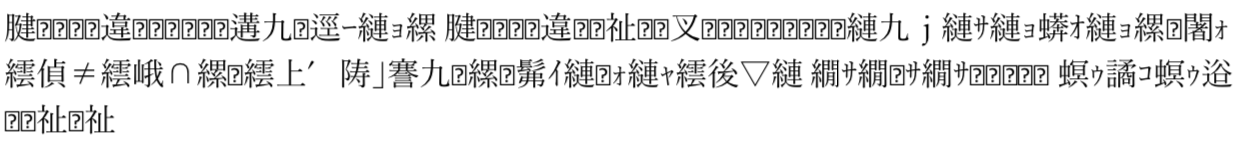
\includegraphics[width=.75\columnwidth]{costlysignaling.png}
\end{figure}
[signal lost]


\chapter*{Afterword}
%!TEX root = main.tex

November 4th, 2019

We are sorry to inform you that the transmission ended here. Like you, we were looking forward to more models about these tri-parental world, such as scaling of cities, cost of signaling, or the emergence of monogamous three person marriages. However, we are extremely honored and grateful to have received this much already. 

We hope you enjoyed this inter-space transmission. 

Postdocs of SFI 


\chapter*{Supplementary Materials}

%\section{Background}

Reproduction is the process by which new organisms are produced by existing organisms. There are a wide variety of reproductive systems that have evolved on Earth and elsewhere, and its evolution depends on its contribution to the fitness of the organism compared to other potential systems. 

Empirically, a reproductive system may consist of several core elements:

\begin{enumerate}

\item \textbf{Sex:} The simplest reproductive system is asexual reproduction. In this case, each individual is capable of independently generating offspring. In the absence of other mechanisms (such as horizontal gene transfer or alternation of generations), each offspring is genetically identical to its parent. Since asexual reproduction does not require any time or energetic cost to finding mates, and all individuals of the population can produce offspring, this strategy can be more efficient and lead to rapid population growth. For example, the asexual reproduction of dandelions (apomixis) on Earth has contributed to its rapid spread. 

Nonetheless, sexual reproduction, where more than one individual is required, is extremely common, both on Earth and elsewhere. This implies that sex can provide strong benefits, since it must overcome the costs of finding mates and coordination among multiple genomes. One important cost of sexual reproduction, first articulated by John Maynard Smith, is the ``two-fold cost of males.'' In cases where sexual reproduction occurs between two sexes, and where only one sex can physically generate offspring, then only half of the population (\emph{i.e.}, only the females) can produce offspring. A mutant that is asexual but otherwise identical to the wildtype organism can on average produce twice as many offspring, since all, rather than half, of its offspring can also produce offspring. Therefore, offspring due to sexual reproduction, where there are two sexes and only one can produce offspring, must, on average, be twice as fit as offspring due to asexual reproduction. 

There are a large number of hypothetical benefits that sexual reproduction can impart on organisms \cite{kondrashov1993classification}. One prominent hypothesis is that sexual reproduction increases the variance of genomes produced in each generation, which can be a bet-hedging strategy in an unpredictable and fluctuating environment. Because sex is so common, it appears that these benefits readily outweigh the ``cost of males'' in many environments. 

\end{enumerate}


\begin{enumerate}
    \item Two-fold cost: ``In an asexual population of stable size, each individual produces an average of one progeny, whereas in a  sexual population with a 1:1 sex ratio each female produces an average of one male and one female progeny. Hence, if a mutation appears causing females to produce two asexual female offspring, its frequency will double in each generation.''~\cite{kondrashov_deleterious_1988}. Also John Maynard SMith, ch. 1, 1978.

    \item Increasing fitness variability /new phenotypes / bringing together good mutations. ``In 1887 Weismann proposed that sex is advantageous because it is 'a source of individual variability furnishing material for  the operation of natural selection. Some data suggest that sexual reproduction can actually cause enhanced fitness of at least a portion of the progeny but the mechanism of this is obscure. Any evolutionary explanation for the maintenance of sexual reproduction can probably fit into Weissmann's framework, because sex does not immediately change allele frequencies and consequently cannot directly improve the popu- lation.''~\cite{kondrashov_deleterious_1988}
    
    \item Mixability~\cite{livnat_mixability_2008}: `` It is commonly believed that, among higher organisms, sexual species (obligate and facultative) are more evolvable than asexual ones (29–31), because they are the founders of wide taxa (12, 29) and are vastly more common (4, 32), while obligate asexuals are mostly recent derivations from sexual ancestors (referred to as ‘’evolutionary dead-ends’’; but see ref. 33) and are phylogenetically sparse (12, 29).”
    
    \item Advantage: removing deleterious mutations. This is the K-model ~\cite{kondrashov_deleterious_1988}.

% From~\cite{power_forces_1976}, ``several plausible models for the evolution of sexuality in multicellular organisms (Williams and Mitton 1973; Williams 1975)''.  But also: ``But multiple mating types would not persist if conditions in each habitat patch were too predictable, for then asexual reproduction would be favored because all asexually produced progeny would be adapted to their habitats while many sexually produced individuals would not.''

\end{enumerate}


\textbf{Number of parents}: For species that reproduce by sexual reproduction, on Earth it is overwhelmingly common for there to be two parents. In other words, genetic material from two individuals combine in order to produce the offspring's genome. While our own life history involves three parents (where the genetic material from three individuals combines to form an offspring, known as triparentalism), this is exceedingly rare on Earth. 

It's not that often discussed or thought about, but sex doesn't have to involve just two parents.  When a zygote is from three parents, it is called \emph{triparentalism}  [OTHER PERRY AND OTHER CITES].  More generally, one can have $n$-parentalism.

Biparentalism almost completely dominates all forms of sexual reproduction on earth.  However, two recent counterexamples have been observed [CITES].  Also, viruses can mix together material from more than two [CITES from Perry].  


Why is non-biparentalism so rare?
\begin{enumerate}
\item Power et al, On Forces of Selection in the Evolution of Mating Types, 1976.~\cite{power_forces_1976} (``formation of an n-ploid zygote by simultaneous or consecutive fusion of three or more gametes''): ``So far as I know, there is no organism requiring the fusion of three or more gametes to form a zygote. There is probably no such organism because of the logistical difficulties of assembling three or more individuals of different sex (or mating type) either simultaneously or consecutively, and individuals requiring two or more mating partners for recombination would thus be at a severe disadvantage in terms of energy expenditure and generation time relative to any others which could successfully reproduce with only a single partner. The n-ploid zygotes might also result in inferior individuals because of mechanical difficulty in segregation of alleles during gametogenesis. An n-ploid individual would probably only be superior if heterosis of n-alleles at a single locus yielded a very great advantage, but even this would probably be offset by the low probability of forming offspring with n-alleles at particular loci. For example, only 2 of the offspring of a union of triploids of genotype ABC would also be ABC, whereas 2 of the offspring of a union between diploids of genotype AB would also be AB, assuming no segregation distortion in either case. Thus the superiority of n-allele heterosis would have to be great enough to more than compensate for reduced proportional output of hybrid offspring, and this would probably require an enormous increase in fecundity.''
\item Perry [CITE] argues that thats there's not necessarily coordination costs.
\item Some have argued that machinery is unclear for it. But not clear that it couldn't be easy with another genetic/biomolecular system.  Perry argues that a 1/4, 1/4, 1/2 system would not be that hard.
\item \cite{hurst_why_1996} briefly discussed multi-parentalism.
\end{enumerate}

Cite Perry. We basically use their model.



%	\item Denis Roze, Disentangling the Benefits of Sex, PLoS Bio, 2012: ``Understanding the evolutionary advantage of sexual reproduction remains one of the most fundamental questions in evolutionary biology. Most of the current hypotheses rely on the fact that sex increases genetic variation, thereby enhancing the efficiency of natural selection; an important body of theoretical work has defined the conditions under which sex can be favoured through this effect. Over the last decade, experimental evolution in model organisms has provided evidence that sex indeed allows faster rates of adaptation. A new study on facultatively sexual rotifers shows that increased rates of sex can be favoured during adaptation to new environmental conditions and explores the cause of this effect. The results provide support for the idea that the benefits of increasing genetic variation may compensate for the short-term costs of sexual reproduction.'' 




\textbf{Mating types:} A subgroup of individuals in a species, which can mate sexually with other subgroups in a systematic pattern.  Review of possible mating type systems, and their combinatorics~\cite{bull_combinatorics_1989}. Emphasizes that vast majority of systems consists of $K$ types, where each type can mate with all other $K-1$ types but not themselves (\emph{self-avoidance}).


%Explain self-avoidance: we have $n$ mating types, who cannot mate with themselves but (usually) all others~\cite{bull_combinatorics_1989}.


If self-avoidance exists, and there is essentially random mixing of mating types, then less common mating types (who can mate with all) will be favored relative to more common mating types,  due to frequency-dependent selection. Absent other effects, this will cause the number of mating types to rise to $n\to \infty$.  This is summarized in a dynamical model by \cite{iwasa_evolution_1987}. This logic is also mentioned earlier, in an informal way, in \cite{power_forces_1976} (`` But if more and more new types were added, each individual would approach universal acceptability and the number of types could come to equal the number of clones.''). Presumably, this will only increase in strength when number of parents to make an offspring increases.

Why do we only observe only two mating types?  Hurst suggests (a somewhat complicated) reason in ~\cite{hurst_why_1996}.  The basic logic (as we understand it) is that it is advantageous to have a single parent contribute the cytoplasm.  With more than two parents, it becomes difficult to guard against selfish mutants, in which two of the parents contribute cytoplasm.  Supports with evidence and citations showing that isogamous systems where mating involves only exchange of nuclear material hundreds or even thousands of mating types can exist.

Power on why not having too many types: ``The maximum number of mating types should be limited by (a) selection against genetically incompatible pairings, (b) competition between members of different mating types, and (c) the between-sexes-choice form of sexual selection operating against genetically incompatible and/or competitively inferior individuals.''~\cite{power_forces_1976}.

Power~\cite{power_forces_1976}: ``In order to understand the selective factors involved in the evolution of mating types, I consider three questions: (1) Why have mating types evolved? (2) Why have more than two types evolved in some populations? (3) What limits the number of types?''



\textbf{Asymmetry}: isogamy vs anisogamy (?). Why do gametes differentiate into one being big (female) and one being small (male)?  This is thought to be the origin of various other sexual dimorphisms.


%Fundamentally, for $n$-parental systems to evolve under natural selection (where $n \geq 3$), it must outcompete other reproductive systems. 



Assume we have $n$ parents and $m$ mating types.  Should we expect to see a symmetry breaking, where the $m$ types are all phenotypically different?


From Power~\cite{power_forces_1976}: ``Parker et al. (1972) have elegantly shown that anisogamy is favored among multicellular organisms if increases in zygote volume produce disproportionately great increases in zygote fitness, but not so much that the benefits of gamete productivity are eliminated. Applying their ideas to protists should yield the same result, i.e., more or less inevitable evolution of anisogamy. What then accounts for the prevalence of isogamy in eucaryotic protists? Probably more constraints are placed on an organism's relative size than a gamete's because it must survive a longer period of time under more variable and less predictable conditions, and thus there may often be but a single optimum size (Parker et al. 1972). Despite the uncommoness of anisogamy among protists, I think it profitable to search for the origin of sexual dimorphism at the protist level because of the possibility anisogamy is primitive with metazoa.''



%!TEX root = main.tex

% Benefit of sex stuff here

\section{An Explanation of Our Triparental System}

Here we review the origin and structure of the $n$-parent system.


\subsection{Why are there $n$ Mating Types?}



From WP, criticisms of \cite{kondrashov_deleterious_1988}: ``There has been much criticism of Kondrashov's theory, since it relies on two key restrictive conditions. The first requires that the rate of deleterious mutation should exceed one per genome per generation in order to provide a substantial advantage for sex. While there is some empirical evidence for it (for example in Drosophila[44] and E. coli[45]), there is also strong evidence against it. Thus, for instance, for the sexual species Saccharomyces cerevisiae (yeast) and Neurospora crassa (fungus), the mutation rate per genome per replication are 0.0027 and 0.0030 respectively. For the nematode worm Caenorhabditis elegans, the mutation rate per effective genome per sexual generation is 0.036.[46] Secondly, there should be strong interactions among loci (synergistic epistasis), a mutation-fitness relation for which there is only limited evidence.[47] Conversely, there is also the same amount of evidence that mutations show no epistasis (purely additive model) or antagonistic interactions (each additional mutation has a disproportionally small effect).'' --- so it works well for high mutation rates and synergistic epistasis --- maybe because their genetic system is system?




%\chapter{Biological Foundations}


%\section{Why are the Mating Types Asymmetric?}
%%!TEX root = main.tex


Our dominant species has three distinct biological sexes, unlike yours, \emph{homo sapiens}, which has two. As with \emph{home sapiens}, there exists asymmetry and this asymmetry has important consequences for the physical traits of our (and your) species, which in turn has consequences for the organization of our society. Here, we provide a model of gamete asymmetry as an Evolutionarily Stable Strategy (ESS).

% TODO: Determine better names for these species.
Let $m_F$, $m_P$, and $m_C$ be the gamete sizes of our Flower, Pollinator, and Central species. We assume a minimum viable gamete size, $m_0$, and represent the ESS gamete sizes by  $m^*_F$, $m^*_P$, and $m^*_C$. The overall viability, $b$, of the double fertilized ``egg'' is a function of the sum of the gamete sizes, $b=b(m_F,m_P,m_C)$. There are three relevant functions, corresponding to a mutant of each sex attempting to invade the ESS, $W_F(m_F,m_F^*,m_P^*,m_C^*)$, $W_P(m_P,m_F^*,m_P^*,m_C^*)$, and $W_C(m_C,m_F^*,m_P^*,m_C^*)$. While this could be analyzed using the Karush–Kuhn–Tucker (KKT) conditions, the problem is simple enough to intuit the relevant inequalities to enforce where constraints -- notably boundary conditions -- exist.

For simplicity, we assume that each $P$ and $C$ individual follows either a single- or double-mating strategy, and that the probability of each sex adopting a double-mating strategy is, respectively, $q^{(P)}$ and $q^{(C)}$. Given this, each ``mating'' of an $F$ individual faces fertilization competition with probability $p^{(P)} = \frac{2 q^{(P)}}{1+q^{(P)}}$ and each mating of a $P$ individual faces fertilization competition with probability $p^{(C)} = \frac{2 q^{(C)}}{1+q^{(C)}}$. We first consider the ESS condition for $F$ individuals, who adopt a gamete size near the minimum viable size.

Consider now the branching probabilities in Table~\ref{tab:branching} for ``matings''. Whereas increasing gamete size improves the viability of offspring, it reduces the amount of sperm competing in each mating, and we assume that the weighting in this competition is inversely proportional to the gamete size (c.f. Parker). Hence, the fitness of an $F$ mutant following strategy $m_F$ while the others follow $m_P^*$ and $m_C^*$ is

% k1 = 1 - P/2 - C/2 + C*P/6 + C*P^2/12
% k2 = P/2 + C/2 - C*P/6 - C*P^2/12
%\begin{equation}
%  \label{eq:W_F}
%  W(m_F,m_P^*,m_C^*) = b(m_F,m_P^*,m_C^*) %\left[(1-p^{(C)})(1-p^{(P)}) + (1-p^{(C)}) p^{(P)} \frac{1}{\frac{m_F}}{\frac{1}{m_F^*} + \frac{1}{m^*_F} \right]
%\end{equation}
\begin{align}
  \label{eq:W_F}
  W_F(m_F,m_P^*,m_P^*,m_C^*) &= b(m_F,m_P^*,m_C^*)  & \nonumber \\ 
  &\big[& \nonumber \\
  &(1-p^{(C)}) \, (1-p^{(P)})& \nonumber \\
  &+(1-p^{(C)}) \, p^{(P)}& \omega(m_F,m_F^*,1) \nonumber \\
  &+p^{(C)} \, (1-p^{(P)}) \, (1-p^{(P)})& \omega(m_F,m_F^*,1) \nonumber \\
  &+p^{(C)} \, (1-p^{(P)}) \, p^{(P)}& \omega(m_F,m_F^*,2) \nonumber \\
  &+p^{(C)} \, p^{(P)} \, (1-p^{(P)})& \omega(m_F,m_F^*,2) \nonumber \\
  &+p^{(C)} \, p^{(P)} \, p^{(P)} & \omega(m_F,m_F^*,3) \nonumber \\
  &\big]
  %&\frac{1}{m_F} \frac{1}{m_F^*} + \frac{1}{m^*_F} ] 
\end{align}

\noindent where for convenience we define the function $\omega$,
\begin{align*}
\omega(m,m^*,\alpha) = \frac{ \frac{1}{m} }{ \frac{1}{m}+\frac{\alpha}{m^*} }.
\end{align*}

\noindent The first derivative of $\omega$ with respect to $m$ is
\begin{align*}
    \frac{\partial \omega}{\partial m} &= \frac{ -\frac{1}{m^2} }{ \frac{1}{m}+\frac{\alpha}{m^*} }+ \frac{ \frac{1}{m^3} }{ [\frac{1}{m}+\frac{\alpha}{m^*}]^2 }\\
    &=-\frac{1}{m}\omega(m,m^*,\alpha)(1-\omega(m,m^*,\alpha)).
\end{align*}

\noindent Evaluating $\omega$ at $m=m^*$ yields

\begin{align*}
    \omega(m^*,m^*,\alpha) = \frac{1}{1+\alpha}.
\end{align*}
Therefore,
\begin{align*}
  \frac{\partial \omega}{\partial m}|_{m=m^*} &=  -\frac{\alpha}{m^*(1+\alpha)}. 
\end{align*}


%\noindent Let 
%\begin{align*}
%    k_1(p^{(C)}, p^{(P)}) = \frac{p^{(C)} (p^{(P)})^2 }{12} %-\frac{5}{6}p^{(C)}p^{(P)}+\frac{p^{(C)}+p^{(P)}}{2}
%\end{align*}
%and
%\begin{align*}
%    k_2(p^{(C)}, p^{(P)}) = \frac{p^{(C)} (p^{(P)})^2 }{12} %+\frac{1}{6}p^{(C)}p^{(P)}-\frac{p^{(C)}+p^{(P)}}{2}.
%\end{align*}
The first derivative of the $W_F$ with respect to $m_F$ evaluated at $m_F=m_F^*$ is
\begin{align}
    \label{eq:cond_F}
    \frac{\partial W}{\partial m_F}|_{m_F=m_F^*} =
    k_1 \, b'(m^*) - \frac{1}{m_F^*} \, k_2 \, b(m^*)
\end{align}

\noindent where

\begin{equation}
  k_1 = 1 - \frac{p_P + p_C}{2} + \frac{1}{6} p_P p_C + \frac{1}{12} p_P^2 p_C
\end{equation}

\noindent and

\begin{equation}
  k_2 = \frac{p_P + p_C}{2} - \frac{1}{6} p_P p_C - \frac{1}{12} p_P^2 p_C \mbox{.}
\end{equation}

\begin{center}
\begin{tabular}{ |r|r|r|c|c|c| } 
 \hline
             &             && $N_C$ & $N_P$ & $N_F$ \\ 
 $1-p^{(C)}$ & $1-p^{(P)}$ && 1     & 1     & 1 \\ 
 $1-p^{(C)}$ &   $p^{(P)}$ && 1     & 1     & 2 \\ 
   $p^{(C)}$ & $1-p^{(P)}$ & $1-p^{(P)}$ & 1     & 2     & 2 \\ 
   $p^{(C)}$ & $1-p^{(P)}$ & $p^{(P)}$ & 1     & 2     & 3 \\ 
   $p^{(C)}$ & $p^{(P)}$ & $1-p^{(P)}$ & 1     & 2     & 3 \\ 
   $p^{(C)}$ & $p^{(P)}$ & $p^{(P)}$ & 1     & 2     & 4 \\ 
 \hline
\end{tabular}
\label{tab:branching}
\end{center}

\noindent Since $m_F^*=m_0$ at the ESS, the following inequality constraint must be satisfied:
\begin{equation}
  \label{eq:W_F}
    \frac{\partial W_F}{\partial m_F}|_{m_F=m_F^*} < 0 \mbox{.}
\end{equation}
Invoking the so-called Marginal Value Theorem (reference Charnov and Parker here), the optimal investment in offspring viability is achieved when the following condition on overall gamete size is satisfied:

\begin{equation}
  \label{eq:mvt}
  b'(m^*) = \frac{b(m^*)}{m^*} \mbox{.}
\end{equation}

\noindent Combining Equations~\ref{eq:cond_F}, \ref{eq:W_F}, and~\ref{eq:mvt}, the optimal gamete size for $F$ is $m_F^*=m_0$ so long as the following inequality is satisfied:

\begin{equation}
  \label{eq:inequa_F}
  \frac{m_F^*}{m^*} < \frac{k_2}{k_1} = \frac{\frac{p_P + p_C}{2} - \frac{1}{6} p_P p_C - \frac{1}{12} p_P^2 p_C }{ 1 - \frac{p_P + p_C}{2} + \frac{1}{6} p_P p_C + \frac{1}{12} p_P^2 p_C} \mbox{.}
  %\frac{m_F^*}{m^*} < -\frac{k_1}{k_2} = -\frac{ \frac{p^{(C)} (p^{(P)})^2 }{12} -\frac{5}{6}p^{(C)}p^{(P)}+\frac{p^{(C)}+p^{(P)}}{2}}{\frac{p^{(C)} (p^{(P)})^2 }{12} +\frac{1}{6}p^{(C)}p^{(P)}-\frac{p^{(C)}+p^{(P)}}{2}}
\end{equation}


% (1-pC) * (1-pP) N_f



%Although temporally $P$ first retrieves genetic material from one or two F's, then delivers this genetic material to one $C$, it is easier to assess the probabilities in reverse temporal order given the probability 
%of fertilization amounts. The probability of genetic material getting delivered to $C$ with only three individuals represented, which symbolically we shall represent by $\{F:1,P:1,C:1\}$ is $p^{(C)} \. p^{(P)}$. 

%single mating for both $C$

%and competition for each species-specific decision about whether to double- or single-mate. With probability $$
%Given the assumption of only single- or double-mating, the probability of each 

\noindent A similar derivation can be applied to $P$, but with the number $N_P$ standing in for $N_F$ in Table~\ref{tab:branching}. One conclude that

\begin{equation}
  \label{eq:inequa_P}
  \frac{m_P^*}{m^*} < \frac{k_2}{k_1} = \frac{1}{\frac{2}{p_C}-1} \mbox{.}
  %\frac{m_F^*}{m^*} < -\frac{k_1}{k_2} = -\frac{ \frac{p^{(C)} (p^{(P)})^2 }{12} -\frac{5}{6}p^{(C)}p^{(P)}+\frac{p^{(C)}+p^{(P)}}{2}}{\frac{p^{(C)} (p^{(P)})^2 }{12} +\frac{1}{6}p^{(C)}p^{(P)}-\frac{p^{(C)}+p^{(P)}}{2}}
\end{equation}

%!TEX root = main.tex


Our dominant species has three distinct biological sexes, unlike yours, \emph{homo sapiens}, which has two. As with \emph{home sapiens}, there exists asymmetry and this asymmetry has important consequences for the physical traits of our (and your) species, which in turn has consequences for the organization of our society. Here, we provide a model of gamete asymmetry as an Evolutionarily Stable Strategy (ESS).

% TODO: Determine better names for these species.
Let $m_F$, $m_P$, and $m_C$ be the gamete sizes of our Flower, Pollinator, and Central species. We assume a minimum viable gamete size, $m_0$, and represent the ESS gamete sizes by  $m^*_F$, $m^*_P$, and $m^*_C$. The overall viability, $b$, of the double fertilized ``egg'' is a function of the sum of the gamete sizes, $b=b(m_F,m_P,m_C)$. There are three relevant functions, corresponding to a mutant of each sex attempting to invade the ESS, $W_F(m_F,m_F^*,m_P^*,m_C^*)$, $W_P(m_P,m_F^*,m_P^*,m_C^*)$, and $W_C(m_C,m_F^*,m_P^*,m_C^*)$. While this could be analyzed using the Karush–Kuhn–Tucker (KKT) conditions, the problem is simple enough to intuit the relevant inequalities to enforce where constraints -- notably boundary conditions -- exist.

For simplicity, we assume that each $P$ and $C$ individual follows either a single- or double-mating strategy, and that the probability of each sex adopting a double-mating strategy is, respectively, $q^{(P)}$ and $q^{(C)}$. Given this, each ``mating'' of an $F$ individual faces fertilization competition with probability $p^{(P)} = \frac{2 q^{(P)}}{1+q^{(P)}}$ and each mating of a $P$ individual faces fertilization competition with probability $p^{(C)} = \frac{2 q^{(C)}}{1+q^{(C)}}$. We first consider the ESS condition for $F$ individuals, who adopt a gamete size near the minimum viable size.

Consider now the branching probabilities in Table~\ref{tab:branching} for ``matings''. Whereas increasing gamete size improves the viability of offspring, it reduces the amount of sperm competing in each mating, and we assume that the weighting in this competition is inversely proportional to the gamete size (c.f. Parker). Hence, the fitness of an $F$ mutant following strategy $m_F$ while the others follow $m_P^*$ and $m_C^*$ is

% k1 = 1 - P/2 - C/2 + C*P/6 + C*P^2/12
% k2 = P/2 + C/2 - C*P/6 - C*P^2/12
%\begin{equation}
%  \label{eq:W_F}
%  W(m_F,m_P^*,m_C^*) = b(m_F,m_P^*,m_C^*) %\left[(1-p^{(C)})(1-p^{(P)}) + (1-p^{(C)}) p^{(P)} \frac{1}{\frac{m_F}}{\frac{1}{m_F^*} + \frac{1}{m^*_F} \right]
%\end{equation}
\begin{align}
  \label{eq:W_F}
  W_F(m_F,m_P^*,m_P^*,m_C^*) &= b(m_F,m_P^*,m_C^*)  & \nonumber \\ 
  &\big[& \nonumber \\
  &(1-p^{(C)}) \, (1-p^{(P)})& \nonumber \\
  &+(1-p^{(C)}) \, p^{(P)}& \omega(m_F,m_F^*,1) \nonumber \\
  &+p^{(C)} \, (1-p^{(P)}) \, (1-p^{(P)})& \omega(m_F,m_F^*,1) \nonumber \\
  &+p^{(C)} \, (1-p^{(P)}) \, p^{(P)}& \omega(m_F,m_F^*,2) \nonumber \\
  &+p^{(C)} \, p^{(P)} \, (1-p^{(P)})& \omega(m_F,m_F^*,2) \nonumber \\
  &+p^{(C)} \, p^{(P)} \, p^{(P)} & \omega(m_F,m_F^*,3) \nonumber \\
  &\big]
  %&\frac{1}{m_F} \frac{1}{m_F^*} + \frac{1}{m^*_F} ] 
\end{align}

\noindent where for convenience we define the function $\omega$,
\begin{align*}
\omega(m,m^*,\alpha) = \frac{ \frac{1}{m} }{ \frac{1}{m}+\frac{\alpha}{m^*} }.
\end{align*}

\noindent The first derivative of $\omega$ with respect to $m$ is
\begin{align*}
    \frac{\partial \omega}{\partial m} &= \frac{ -\frac{1}{m^2} }{ \frac{1}{m}+\frac{\alpha}{m^*} }+ \frac{ \frac{1}{m^3} }{ [\frac{1}{m}+\frac{\alpha}{m^*}]^2 }\\
    &=-\frac{1}{m}\omega(m,m^*,\alpha)(1-\omega(m,m^*,\alpha)).
\end{align*}

\noindent Evaluating $\omega$ at $m=m^*$ yields

\begin{align*}
    \omega(m^*,m^*,\alpha) = \frac{1}{1+\alpha}.
\end{align*}
Therefore,
\begin{align*}
  \frac{\partial \omega}{\partial m}|_{m=m^*} &=  -\frac{\alpha}{m^*(1+\alpha)}. 
\end{align*}


%\noindent Let 
%\begin{align*}
%    k_1(p^{(C)}, p^{(P)}) = \frac{p^{(C)} (p^{(P)})^2 }{12} %-\frac{5}{6}p^{(C)}p^{(P)}+\frac{p^{(C)}+p^{(P)}}{2}
%\end{align*}
%and
%\begin{align*}
%    k_2(p^{(C)}, p^{(P)}) = \frac{p^{(C)} (p^{(P)})^2 }{12} %+\frac{1}{6}p^{(C)}p^{(P)}-\frac{p^{(C)}+p^{(P)}}{2}.
%\end{align*}
The first derivative of the $W_F$ with respect to $m_F$ evaluated at $m_F=m_F^*$ is
\begin{align}
    \label{eq:cond_F}
    \frac{\partial W}{\partial m_F}|_{m_F=m_F^*} =
    k_1 \, b'(m^*) - \frac{1}{m_F^*} \, k_2 \, b(m^*)
\end{align}

\noindent where

\begin{equation}
  k_1 = 1 - \frac{p_P + p_C}{2} + \frac{1}{6} p_P p_C + \frac{1}{12} p_P^2 p_C
\end{equation}

\noindent and

\begin{equation}
  k_2 = \frac{p_P + p_C}{2} - \frac{1}{6} p_P p_C - \frac{1}{12} p_P^2 p_C \mbox{.}
\end{equation}

\begin{center}
\begin{tabular}{ |r|r|r|c|c|c| } 
 \hline
             &             && $N_C$ & $N_P$ & $N_F$ \\ 
 $1-p^{(C)}$ & $1-p^{(P)}$ && 1     & 1     & 1 \\ 
 $1-p^{(C)}$ &   $p^{(P)}$ && 1     & 1     & 2 \\ 
   $p^{(C)}$ & $1-p^{(P)}$ & $1-p^{(P)}$ & 1     & 2     & 2 \\ 
   $p^{(C)}$ & $1-p^{(P)}$ & $p^{(P)}$ & 1     & 2     & 3 \\ 
   $p^{(C)}$ & $p^{(P)}$ & $1-p^{(P)}$ & 1     & 2     & 3 \\ 
   $p^{(C)}$ & $p^{(P)}$ & $p^{(P)}$ & 1     & 2     & 4 \\ 
 \hline
\end{tabular}
\label{tab:branching}
\end{center}

\noindent Since $m_F^*=m_0$ at the ESS, the following inequality constraint must be satisfied:
\begin{equation}
  \label{eq:W_F}
    \frac{\partial W_F}{\partial m_F}|_{m_F=m_F^*} < 0 \mbox{.}
\end{equation}
Invoking the so-called Marginal Value Theorem (reference Charnov and Parker here), the optimal investment in offspring viability is achieved when the following condition on overall gamete size is satisfied:

\begin{equation}
  \label{eq:mvt}
  b'(m^*) = \frac{b(m^*)}{m^*} \mbox{.}
\end{equation}

\noindent Combining Equations~\ref{eq:cond_F}, \ref{eq:W_F}, and~\ref{eq:mvt}, the optimal gamete size for $F$ is $m_F^*=m_0$ so long as the following inequality is satisfied:

\begin{equation}
  \label{eq:inequa_F}
  \frac{m_F^*}{m^*} < \frac{k_2}{k_1} = \frac{\frac{p_P + p_C}{2} - \frac{1}{6} p_P p_C - \frac{1}{12} p_P^2 p_C }{ 1 - \frac{p_P + p_C}{2} + \frac{1}{6} p_P p_C + \frac{1}{12} p_P^2 p_C} \mbox{.}
  %\frac{m_F^*}{m^*} < -\frac{k_1}{k_2} = -\frac{ \frac{p^{(C)} (p^{(P)})^2 }{12} -\frac{5}{6}p^{(C)}p^{(P)}+\frac{p^{(C)}+p^{(P)}}{2}}{\frac{p^{(C)} (p^{(P)})^2 }{12} +\frac{1}{6}p^{(C)}p^{(P)}-\frac{p^{(C)}+p^{(P)}}{2}}
\end{equation}


% (1-pC) * (1-pP) N_f



%Although temporally $P$ first retrieves genetic material from one or two F's, then delivers this genetic material to one $C$, it is easier to assess the probabilities in reverse temporal order given the probability 
%of fertilization amounts. The probability of genetic material getting delivered to $C$ with only three individuals represented, which symbolically we shall represent by $\{F:1,P:1,C:1\}$ is $p^{(C)} \. p^{(P)}$. 

%single mating for both $C$

%and competition for each species-specific decision about whether to double- or single-mate. With probability $$
%Given the assumption of only single- or double-mating, the probability of each 

\noindent A similar derivation can be applied to $P$, but with the number $N_P$ standing in for $N_F$ in Table~\ref{tab:branching}. One conclude that

\begin{equation}
  \label{eq:inequa_P}
  \frac{m_P^*}{m^*} < \frac{k_2}{k_1} = \frac{1}{\frac{2}{p_C}-1} \mbox{.}
  %\frac{m_F^*}{m^*} < -\frac{k_1}{k_2} = -\frac{ \frac{p^{(C)} (p^{(P)})^2 }{12} -\frac{5}{6}p^{(C)}p^{(P)}+\frac{p^{(C)}+p^{(P)}}{2}}{\frac{p^{(C)} (p^{(P)})^2 }{12} +\frac{1}{6}p^{(C)}p^{(P)}-\frac{p^{(C)}+p^{(P)}}{2}}
\end{equation}

% Dynamical model for Gamete asymetry in 2 and 3 sexes (Vicky's)
\begin{figure}
    \centering
    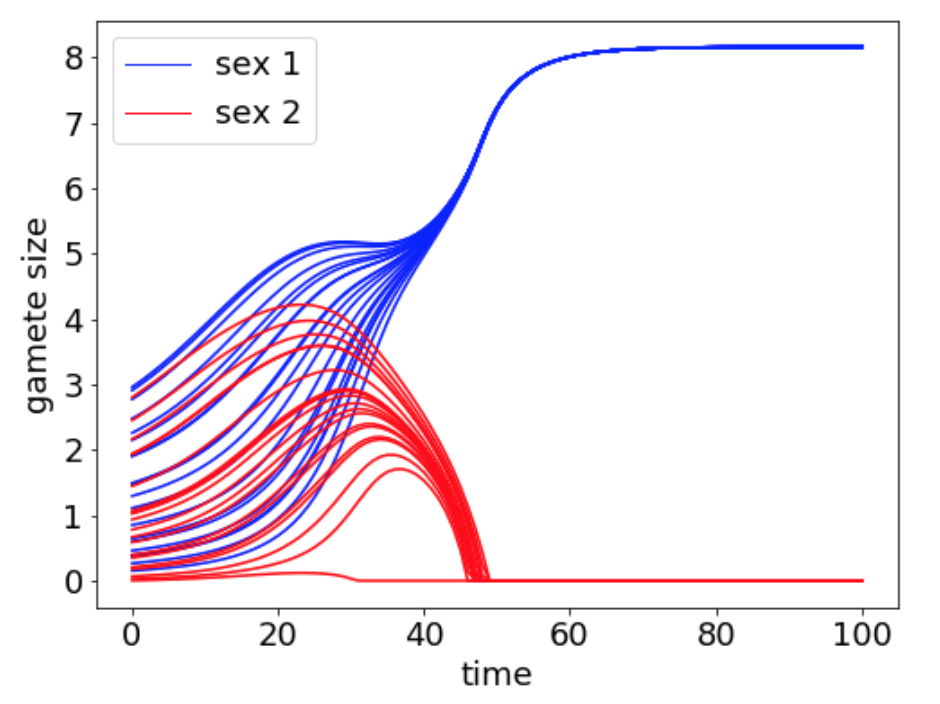
\includegraphics[width = 0.6\textwidth]{vickysFigs/2_sex_run1.png}
    \caption{Simulation for the gamete size evolution in the case of two sexes. One sex evolves to have the minimal size gametes (0, in this model), and the other sex evolves to have large gametes.}
    \label{fig:my_label}
\end{figure}

\section*{Genetics}
%Main text
As mentioned above, we thought it would be helpful for you to get a basic overview of how our genetic system differs from yours. The important distinction to remember is that our species have a triploid genome that is made from combining three haploid gametes from our three parents (each of a distinct self-avoiding mating type), as opposed to your diploid genome that is made from combining two haploid gametes from your two parents.

\subsection{Recombination and gamete formation}

Each of our mating types makes a haploid gamete. The genetic material in this gamete is a third of the genetic material of its producer. Importantly, there is a recombination event that occurs before production of the gametes to ensure that there is genetic variation


\subsection{Determining mating type}

\subsection{Gene expression}



%in abstract
The details of the origin of the biochemistry of our life form, as well as the precise chemistry that forms it, will be discussed in a later section. Here we will focus on explaining our genetics and how it compares to the genetics of your species. For this reason we will talk about our genetic material as sets of double stranded chromosomes so that you are able to understand the analogy. The main distinction however, is that unlike your diploid genomes, where you inherit one copy of each chromosome from one of your two parents, our genome is triploid, where we inherit one copy of each chromosome from one of our three parents. The details of the recombination events occurring pre-gamete formation are discussed in the 'genetics textbook' part of the SI and an overview is shown in Figure .

The dynamics of our genetics and how it affects assignment of mating types is surprisingly analogous to yours, but with some key differences which will be expanded upon in the SI. As discussed previously, our species is composed of three mating types. These mating types are distinguished by three sex-determining genotypes: 'XXY', 'XYY' and 'XYZ'. Each of these mating types produce haploid gametes, and all three gametes need to come together in order to produce a triploid off-spring. Each parent thus contributes a third of its genetic material to the offspring and conversely the offpring's genome is composed of a third of each of its parents genome. The XYZ mating type produces the largest gamete, that is then fertilized by the other two smaller ones. In your species, you would thus define XYZ as female and the other two as different types of males, although it is important to note that this analogy does not quite match with our genders. The main difference to note is that the two 'male' mating-types each produce only one type of gamete. The XXY genotype only produces X gametes while the XYY genotype only produces Y gametes. It follows that the female, producing all three X, Y and Z gametes, is the one that biologically determines the mating type of the offspring. We have included an extension of a "Punnet square" to illustrate this concept in Table. 


\section*{Families}
%!TEX root = main.tex




% [maybe to add somewhere else?] One notable exception is among more recent in-vitro fertilization (IVF) couples, where genetic material from two eggs may be combined with that of one sperm. The most common historic combination of more than 2 individuals in a family composes one male and multiple females.

% question, describe marriage here or in the introduction? 


%[this would have been interesting if we had a model of how monogama emerged within this system using Laura Fortunato's stuff] 

%O

% Moreover, there is evidence on Earth that two-person reproduction leads to great inequality in the division of labor. 

\section*{Matching/Divorce}
%!TEX root = main.tex

% bonding rates

\subsubsection{Background}

While polygyny is the default marriage system, monogamy is common across wealthy nations and is considered the default by much research. According to Fortunato \cite{Fortunato2015, Fortunato2009}, monogomy tends to occur if . In a monogamous society, paternity can be assured due to high investment by fathers. Low investment can lead to unsure paternity. 

We consider the case where individuals need to match with 2 instead of 1 other person. 

Here we present a simple model based on a concept you seem to be comfortable, ``Nash equilibrium''. The population consists of $N$ types of sex, and each sex contains $n$ number of agents. Let $a_{i,s}$ be an agent ID $i$ from sex $s$. Each agent is characterized by its feature $X_{i,s}$. They can form a marriage by find a mate from each other sex. If an agent Their preference for marriage is represented by a utility function $u_{i,s}(X_{})$.

For each period, we repeat the following steps:
\begin{enumerate}
    \item Pick up one person from each sex randomly.
    \item They three consider the utility from their marriage.
    \item If {\textit all} of them think this new marriage is better than their current one, then they each break up the existing marriage and form the new one.
    \item Else, nothing happens.
\end{enumerate}





The divorce-and-marriage constantly happens in our system compared to biparental 

\section*{Health}
%!TEX root = main.tex



\section*{Cultural mixing Under $n$-parental reproduction}
%!TEX root = main.tex

\subsubsection{Background to the Problem}

In this section, we provide a simple probabilistic model for calculating an individual's expected number of cultural affinities, such as language or membership in a legal forming group, and show how it provides evidence for an explanatory role for $3$-parent marriage in the emergence of cultural homogeneity in our society.\par 

Suppose that there are $n$ people in the world. Let a possible world $\omega$ be defined as follows:
\begin{equation}
    \omega = \bigcup_{i=1}^{n}(MICA_{i}, M_{i}, CM_{i}, TCA_{i})
\end{equation}
Each $4$-tuple $(MICA_{i}, M_{i}, CM_{i}, TCA_{i})$ represents one individual in the world. Let $WC$ be the set of cultures in the world, which we assume to have infinite but countable cardinality. $MICA_{i}\subseteq WC$ is the cultural affinities that $i$ has independent of marriage. Let $M_{i}$ be the set of other individuals in the population to whom $i$ have ever married. Marriage is a symmetric and transitive (but not reflexive) relation on the set of individuals. $CM_{i}\subseteq WC$ is defined as follows:
\begin{equation}
    CM_{i}=\bigcup_{j\in M_{i}}MICA_{j}\setminus\bigcap_{j\in M_{i}}MICA_{j}
\end{equation}
In other words, $CM_{i}$ is the set of distinct cultures with which $i$'s spouses have marriage-independent affinities. $CM_{i}$ is empty if and only if the individual $i$ is unmarried, so that $M_{i}$ is empty (this assumes no stateless people). Finally, let $TCA_{i}$ be defined as follows:
\begin{equation}
    TCA_{i}=(MICA_{i}\cup CM_{i})\setminus (MICA_{i}\cap CM_{i})
\end{equation}
In other words, $TCA_{i}$ is $i$'s total set of distinct cultural affinities, both independent of marriage and through marriage.\par 

In each possible world $\omega$, assume that $MICA_{i}$ is i.i.d.\ across individuals. Let us define a probability space $(\Omega,\mathcal{P}(\Omega),P(\cdot))$, where $\mathcal{P}(\Omega)$ is the power set of $\Omega$. Let $[TCA_{i}=\alpha]\in\mathcal{P}(\Omega)$ be the set of possible worlds in which the cardinality of $TCA_{i}$ is $\alpha$, i.e.\ the worlds in which $i$ has $\alpha$ distinct cultural affinities. Let $[CM_{i}=\beta]\in\mathcal{P}(\Omega)$ be the set of possible worlds in which the cardinality of $CM_{i}$ is $\beta$, i.e.\ the worlds in which $i$'s spouses have $\beta$ distinct cultural affinities. We can calculate any individual $i$'s expect cultural affinities:
\begin{equation}
    \mathbbm{E}(C_{i})=\sum_{\alpha=1}^{\infty}\alpha P([TCA_{i}=\alpha])
\end{equation}
The law of total probability gives us:
\begin{equation}
    \mathbbm{E}(C_{i}) =  \sum_{\alpha=1}^{\infty}\sum_{\beta=0}^{\infty}\alpha P([TCA_{i}=\alpha]|[CM_{i}=\beta])P([CM_{i}=\beta])
\end{equation}
Which we expand as follows:
\begin{multline}
    \mathbbm{E}(C_{i})= \sum_{\alpha=1}^{\infty}\alpha\big(P([TCA_{i}=\alpha]|[CM_{i}=0])P([CM_{i}=0]) \\ + \  \sum_{\beta=1}^{\infty} P([TCA_{i}=\alpha]|[CM_{i}=\beta])P([CM_{i}=\beta])\big)
\end{multline}
Let $UM_{i}\in\mathcal{P}(\Omega)$ be the set of worlds in which $i$ never marries. By definition, $UM_{i}=[CM_{i}=0]$. So we can re-write the above as follows:
\begin{equation}
    \mathbbm{E}(C_{i})=\sum_{\alpha=1}^{\infty}\alpha\big(P([TCA_{i}=\alpha]|UM_{i})P(UM_{i}) +  \sum_{\beta=1}^{\infty} P([TCA_{i}=\alpha]|[CM_{i}=\beta])P([CM_{i}=\beta])\big)
\end{equation}
Whenever $i$ has never married, their overall cultural affinities match their marriage-independent cultural affinities. This gives us the following:
\begin{equation}
    P([TCA_{i}=\alpha]|UM_{i})=P([MICA_{i}=\alpha])
\end{equation}
So we can re-write the above as follows:
\begin{equation}
    \mathbbm{E}(C_{i})=\sum_{\alpha=1}^{\infty}\alpha\big(P([MICA_{i}=\alpha])P(UM_{i}) + \sum_{\beta=1}^{\infty} P([TCA_{i}=\alpha]|[CM_{i}=\beta])P([CM_{i}=\beta])\big)
\end{equation}
Finally, applying the law of total probability one more time, we get the following:
\begin{multline}
    \mathbbm{E}(C_{i})=\sum_{\alpha=1}^{\infty}\alpha\big(P([MICA_{i}=\alpha])P(UM_{i}) \\ + \    \sum_{\gamma=1}^{\infty}\sum_{\beta=1}^{\infty} P([TCA_{i}=\alpha]|[CM_{i}=\beta]) P([CM_{i}=\beta]|[MICA_{i}=\gamma])P([MICA_{i}=\gamma])\big)
\end{multline}
Based on historical data from our interplanetary system, the prior probability $P([MICA_{i}=\gamma])$, when the mean value of $\gamma$ is $\mu_{\gamma}$, can be found via the following Poisson function:
\begin{equation}
    P([MICA_{i}=\gamma]) \\ = \ f(\gamma,\mu_{\gamma})=\frac{\mu_{\gamma}^{\gamma}e^{-\mu_{\gamma}}}{\gamma!}
\end{equation}
The value of the probability $P([CM_{i}=\beta]|[MICA_{i}=\gamma])$, for any $\beta$ and $\gamma$ is best estimated by the following Poisson function:
\begin{equation}
    P([CM_{i}=\beta]|[MICA_{i}=\gamma])= g(\beta,\gamma)=\frac{(.05+\gamma)^{\beta}e^{-(.05+\gamma)}}{\beta!}
\end{equation}
Thus, the mean number of distinct cultural affinities of a person's marriage partners increases linearly, albeit very slightly, with one's marriage-independent cultural affinities. This reflects the fact that in our society, as on Earth, marriage partners tend to share cultural affinities \cite{Schwartz2013}. The value of the probability $P([TCA_{i}=\alpha]|[CM_{i}=\beta])$ is best estimated by the following Poisson function:
\begin{equation}
    P([TCA_{i}=\alpha]|[CM_{i}=\beta]) = h(\alpha,\beta)=\frac{(.17+\beta^{1.2})^{\alpha}e^{-(.17+\beta^{1.2})}}{\alpha!}
\end{equation}
Thus, the mean number of a person's cultural affinities increases super-linearly with the number of distinct cultural affinities of their marriage partners.\par 

These findings allow us to re-write the equation for $\mathbbm{E}(C_{i})$ as follows:\ 
\begin{equation}
    \mathbbm{E}(C_{i})=\sum_{\alpha=1}^{\infty}\alpha\big(f(\alpha,\mu_{\gamma})P(UM_{i}) + \sum_{\gamma=1}^{\infty}\sum_{\beta=1}^{\infty} h(\alpha,\beta)g(\beta,\gamma)f(\gamma,\mu_{\gamma})\big)
\end{equation}
At this point, we have a framework within which we can state our hypothesis for the generation of homogeneity in our civilization over time. As shown in Section IV.A, the average person under three-partner marriage is much less likely to never marry over the course of their life, and therefore in much more likely to have several partners. More generally, when the number of simultaneous marriage partners is unrestricted, $P(UM_{i})$ is lower than in cases where individuals are permitted only one simultaneous marriage partner. Further, and perhaps more crucially, the following all hold:\ 
\begin{itemize}
\item $f(\gamma,\mu_{\gamma})$ is such that, for any $\gamma$ and $\epsilon$, the probability that $\gamma>\epsilon$ increases as $\mu_{\gamma}$ increases.

\item $g(\beta,\gamma)$ is such that, for any $\beta$ and $\epsilon$, the probability that $\beta>\epsilon$ increases as $\gamma$ increases.

\item $h(\alpha,\beta)$ is such that, for any $\alpha$ and $\epsilon$, the probability that $\alpha>\epsilon$ increases as $\beta$ increases.

\end{itemize}
Thus, $\mathbbm{E}(C_{i})$ is driven up as $\mu_{\gamma}$ increases, i.e.\ as the average number of cultural affinities that a person acquires independently of marriage increases. In a world in which a child can be created via $n$ parents, and inherits the cultural identity of all these parents, and inter-cultural mating is possible, $\mu_{\gamma}$ increases much faster than in a world with the same amount of inter-cultural exchange, but in which a child can only be created by two parents.\par 






\bibliography{ref}{}
\bibliographystyle{plain}

\clearpage



\end{document}
